\documentclass[journal]{IEEEtran} % use the `journal` option for ITherm conference style
\IEEEoverridecommandlockouts
% The preceding line is only needed to identify funding in the first footnote. If that is unneeded, please comment it out.

\usepackage{hyperref}
\usepackage{cite}
\usepackage{amsmath,amssymb,amsfonts}
\usepackage{algorithmic}
\usepackage{graphicx}
\usepackage{textcomp}
\usepackage{xcolor}
\usepackage{graphicx} % To include images
\usepackage{float} % To use [H] for figure placement
\graphicspath{img}

\def\BibTeX{{\rm B\kern-.05em{\sc i\kern-.025em b}\kern-.08em
    T\kern-.1667em\lower.7ex\hbox{E}\kern-.125emX}}

\begin{document}

\title{Enhanced spectrum sensing for 5G and LTE utilizing Unet-Based deep network}
\author{%%%% author names
    \IEEEauthorblockN{Huan Nguyen-Duy}% first author
    , \IEEEauthorblockN{Thien Huynh-The}% delete this line if not needed
    \\%%%% author affiliations
    \IEEEauthorblockA{Ho Chi Minh City University of Technology and Education}\\
    {Ho Chi Minh City, $70000$, Vietnam}\\% first affiliation
    %%%% corresponding author contact details
    \IEEEauthorblockA{Email: huan$2931$@gmail.com, thienht@hcmute.edu.vn} \\
    % \IEEEauthorblockA{thienht@hcmute.edu.vn}
}
\maketitle

\begin{abstract}
Spectrum sensing for wireless communication has a crucial role in the next generation network, allowing devices to identify and accommodate demand for wireless connectivity. In this paper, we address spectrum sensing challenges and introduce an innovative deep network named spectrum sensing network (SpecSenseNet) to tackle over-the-air communication sensing. We feature an architecture derived from Unet, integrating state-of-the-art approaches to enhance sensing performance, encompassing depthwise separable convolution, recurrent residual block, and Atrous Spatial Pyramid Pooling, which are designed to reduce network complexity while maintaining high predictive performance. Consequently, our design effectively reduces parameters count by $75.1\%$ in comparison to Unet. In terms of evaluation, we generate a synthetic signal dataset of two primary signal types (fifth generation new radio and long-term evolution) that are adapted to various levels of additive noise in the range of $[0, 30]$ dB. Relying on simulation results, our network outperforms impressive results with high performance for spectrum sensing, it maintains excellent precision while reducing significant network complexity. Our implementation and pre-trained model are available at:
\href{https://github.com/Winxkin/Spectrum_sensing_base_on_Deep_learning.git}{Spectrum sensing base on deep learning Github project}
\end{abstract}

\begin{IEEEkeywords}
    spectrum sensing network (SpecSenseNet), spectrum sensing, 5G new radio (5G NR), long-term evolution (LTE), Unet, semantic image segmentation, signal processing.
\end{IEEEkeywords}

\section{Introduction}
\subsection{Spectrum sensing}
Spectrum sensing is defined as identifying the availability and non-availability of wireless communication networks or radio networks in particular frequency bands. When a traditional frequency allocation scheme cannot provide high data rate demand constantly, it leads to waste spectrum resources that can be allocated for others in need, such fifth generation (5G) new radio (NR) or long-term evolution (LTE) simultaneously. Therefore, spectrum sensing for 5G NR and LTE becomes a main topic that contains many challenges, focusing on performance enhancement of monitoring and managing limited spectrum resources effectively. The Fig. \ref{fig1} shows an overview of spectrum sensing for 5G and LTE applications and services.

\begin{figure}[!ht]
    \centering
    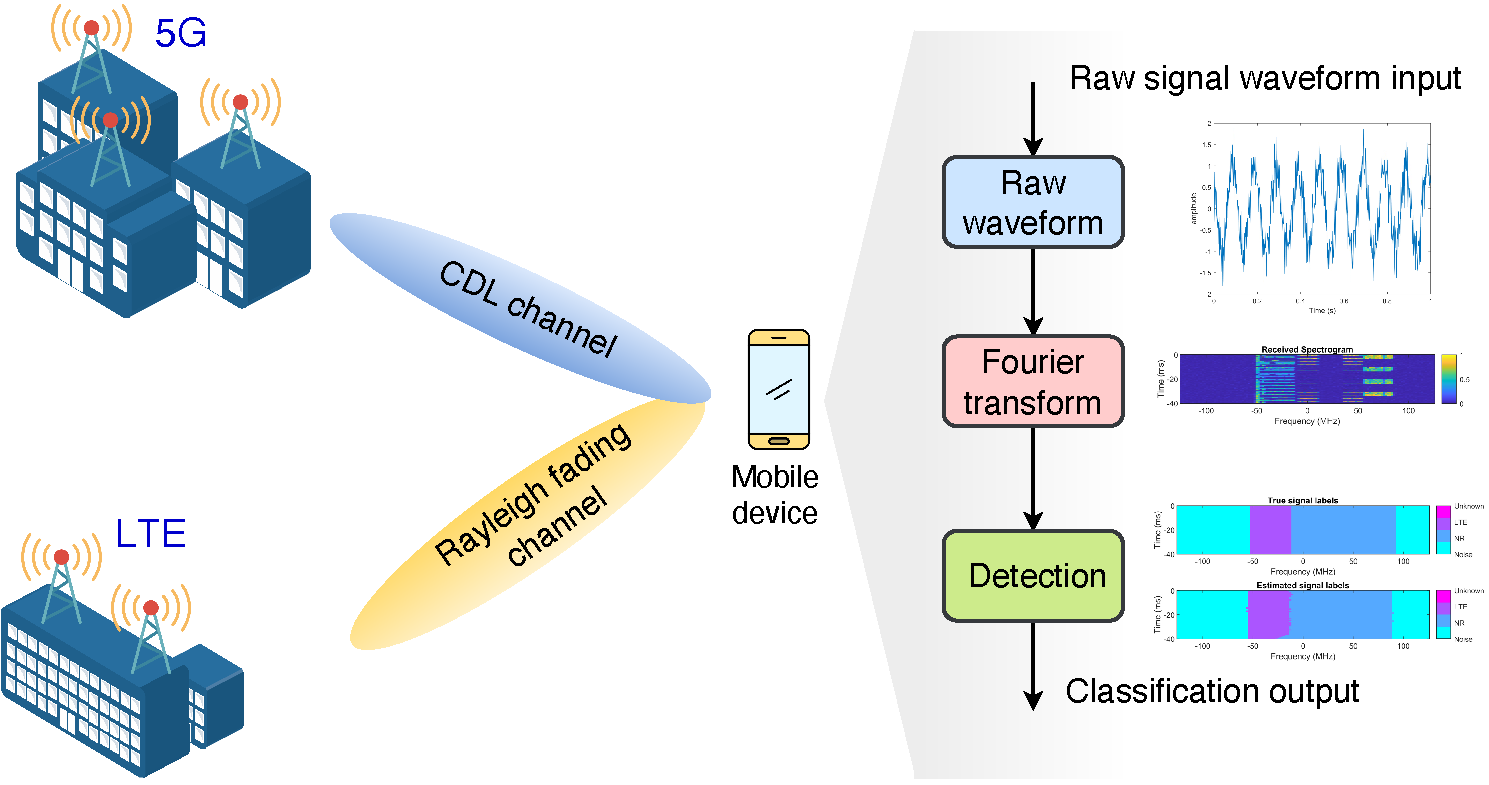
\includegraphics[width=0.45\textwidth]{img/Design-Overview.pdf}
    \caption{Spectrum sensing for 5G and LTE application.}
    \label{fig1}
\end{figure}

In the past, numerous sensing techniques have introduced by using sensing algorithms, multi-dimensional spectrum sensing, channel estimation, and cooperative sensing. Nevertheless, spectrum sensing meets a big challenge in hardware requirements, it requires high sampling rates, high-resolution analog-to-digital converters (ADC) in large dynamic ranges, and high-performance processors~\cite{YucekSpectrumSensing}. On the other hand, cognitive wireless communication can be identified based on sensing duration and frequency~\cite{kumar2024analysis}. However, this method have a trade-off between performance and sensing algorithms. Since their introduction, researchers have spent efforts to tackle improved spectrum sensing problems, addressing various challenges and introducing innovative solutions to increase accuracy and performance in cognitive wireless communication networks. Furthermore, prominent surveys on this topic are introduced in~\cite{ali2016advances} and \cite{liyanaarachchi2021optimized}, in which research directions and machine learning based solutions for intelligent spectrum sensing are investigated and discussed exhaustively.


\subsection{Related work}
In recent years, many works on cognitive wireless communication and radio networks have been introduced to enhance sensing performance. In general, energy detector based sensing is a common approach of spectrum sensing because it offers minimal computation and implementation complexity, waveform-based sensing increases sensing performance, and cyclostationarity-based sensing for detecting and matching filtering primary user transmissions. On the other hand, several innovative deep learning (DL) approaches are presented to tackle spectrum sensing performance. Applying convolutional neural networks for improved waveform classification \cite{huynh2024improved}, the work \cite{huynhthe2023intelligence} introduces an innovative DL architecture to improve the spectrum sensing prediction ratio for 5G and LTE signals. Other works utilize deeplabv3+ \cite{nguyen2023accurate} and DetectNet \cite{gao2019deep} to increase accuracy for spectrum sensing. Nevertheless, while sensing algorithms have a trade-off between hardware performance and computation complexity, DL models offer higher parameters to reach a high level of precision that requires considerable hardware resources.

\subsection{Contribution}
In this work, we exploit DL techniques to tackle sensing tasks and propose an innovative DL architecture based on Unet, called \underline{Spec}trum \underline{Sen}sing \underline{Net}work (SpecSenseNet), which significantly reduces network complexity and enhance sensing performance for 5G and LTE signals. As Unet is a fully convolutional network \cite{ronneberger2015u} for effective semantic image segmentation, it is designed with a parallel encoder-decoder and connected together by skip connections. Recently, Unet++ and other variant models\cite{zhou2019unet++} have shown notable improvements of segmentation accuracy; however, these models consume large memory and expensive computational cost. As a result, they are not suitable for resource-constrained devices. In terms of decreasing network complexity without degradation of segmentation accuracy, we present SpecSenseNet, wherein its architecture incorporates depthwise separable convolutions~\cite{CholletXception} and recurrent residual convolution~\cite{AlomNuclei, he2016deep, aghalari2021brain}, replacing Unet blocks into each layer of encoder and decoder paths. On the other hand, Atrous Pyramid Spatial Pooling (APSS) modules~\cite{ChenAtrous} are adapted to between encoder and decoder paths to enhance relevant feature learning at multiple scales. In summary, we make the following two main contributions:
\begin{itemize}
\item Addressing spectrum sensing for 5G and LTE problems and utilizing DL approaches to tackle spectrum sensing.
\item Introducing an innovative SpecSenseNet architecture based on Unet that reduces significant network complexity and enhances sensing performance for 5G and LTE signals.
\end{itemize}

%%

\section{Methodology}
\subsection{Signal model}
Nowadays, over-the-air communication systems have a vital role in diverse scenarios and applications \cite{lin20215g}. This work mainly considers about 5G NR and LTE communication systems. In practical terms, received signals (called RX signal) from different sources can be defined by (\ref{eq:rxsig}), where $\mathrm{y(t)}$ denotes for the RX signal, $\mathrm{x(t)}$ is the transmitted signal (called TX signal), the channel response $\mathrm{h(t)}$, and $\mathrm{n(t)}$ presents for additive white gaussian noise (AWGN) 

\begin{equation}
    \mathrm{y(t) = x(t) * h(t) + n(t)},
    \label{eq:rxsig}
\end{equation}

\begin{equation}
    \mathrm{Y(\tau, w) = \int_{-\infty}^{\infty} y(t) \cdot w(t - \tau) \cdot e^{-j2\pi ft} \, dt},
    \label{eq:spectrogram}
\end{equation}
\begin{equation}
    \mathrm{E = \sum_{f = f_{\text{min}}}^{f_{\text{max}}} \left| Y(\tau, w) \right|^2}.
    \label{eq:energy}
\end{equation}

\footnotetext[1]{ the operator * represents for convolution operation}

Short-time Fourier transform (STFT) is a widely used signal processing technique for analyzing the frequency content of a signal over time. The RX signal (\ref{eq:rxsig}) can be presented in the frequency domain by STFT that is defined in (\ref{eq:spectrogram}). In detail, $\mathrm{Y(\tau, w)}$ represents the spectrogram of the RX signal at frequency $\mathrm{f}$ and time $\mathrm{t}$, $\mathrm{y(t)}$ is the input RX signal, $\mathrm{w(t - \tau)}$ denotes the window function used for segmenting the signal into short frames. Furthermore, the energy density of signal models is illustrated by the equation (\ref{eq:energy}), with $E$ denotes the energy density in the range of $\mathrm{\left [ f_{\min}, f_{\max} \right ]}$.

Signal-to-noise ratio (SNR) in both 5G and LTE systems can be calculated by comparing the power of the signal to the power of the noise. In wireless communication systems, SNR is typically defined as the ratio of the average received signal power to the average noise power over a specified bandwidth, higher noise ratio means that the level of unwanted interfering signals relative to the desired signal is significant, which can degrade the quality and reliability of data transmission. The signal power depends on factors such as the transmitted power, path loss, antenna gains, and fading effects. In particular, there are several spectrogram generation samples in Fig. \ref{fig2} that present 5G NR, LTE, and overlapping 5G and LTE, respectively.


\begin{figure}[!t]
    \centering
    \footnotesize
    \begin{tabular}{ccc}
        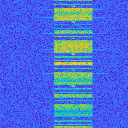
\includegraphics[width=0.13\textwidth]{img/LTE_frame_0.png}  & 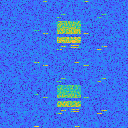
\includegraphics[width=0.13\textwidth]{img/NR_frame_1506.png} &
        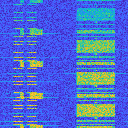
\includegraphics[width=0.13\textwidth]
        {img/LTE_NR_frame_0.png} 
        \\
        (a) & (b) & (c)
    \end{tabular}
    \caption{Spectrogram of received signals: (a) LTE, (b) 5G NR, (c) overlapping 5G NR and LTE}
    \label{fig2}
\end{figure}

\subsection{SpecSenseNet: A robust and cost-efficient deep network}
In this work, we propose the SpecSenseNet that is defined as a robust and cost-efficient convolution network utilizing Unet-Based architecture \cite{ronneberger2015u}. In general, this work utilizes depthwise separable convolution (DSC) \cite{CholletXception} as a convolution operation that replaced for traditional convolutions. DSC uses inoperative depthwise convolution and pointwise convolution to reduce significant the number of convolution operators. The out of DSC can be illustrated in the formula (\ref{eq:Fdsc}), while $\mathrm{F_{\text{DSC}}}$ denotes for the output of DSC with the number of features maps $\mathrm{F_{\text{in}}}$, $\mathrm{dwconv}$ represents for depthwise convolution, following by batch normalization ($\mathrm{bn}$), pointwise convolution ($\mathrm{pconv}$), and relu activation function ($\mathrm{relu}$), respectively

\begin{equation}
    \mathrm{F_{\text{DSC}}(F_{in}) = relu(pconv(bn(dwconv(F_{in}))))}.
    \label{eq:Fdsc}
\end{equation}

On the other hand, this work applies Atrous Spatial Pyramid Pooling (ASPP) \cite{ChenAtrous} into between encoder and decoder paths of SpecSenseNet to enhance the ability of feature extractions in multiple scales. ASPP incorporate parallel four convolution layers, which include a $\mathrm{1\times1}$ convolution layer and three $\mathrm{3\times3}$ convolution layers in different dilatation rates. The output of ASPP is synthesized by a concatenation layer. The Fig. \ref{fig3} depicts ASPP module, with $\mathrm{r_1, r_2, r_3}$ represent for dilatation rates of three $\mathrm{3\times3}$ convolution layers. 


The output of ASPP module can be calculated by (\ref{eq:ASPP}), with $\mathrm{F_{\text{ASPP}}}$ illustrates for the output of ASPP module, while $\mathrm{r_1, r_2, r_3}$ represent dilatation rates, $\mathrm{F_{in}}$ indicates for the number of input feature maps. Furthermore, $\mathrm{F_{\text{Concat}}}$ denotes the output of the concatenation operation and $mathrm{conv}$ denotes convolution layers, respectively

\begin{equation}
\begin{aligned}
    \mathrm{F_{\text{ASPP}}(F_{in},r_1,r_2,r_3) = F_{\text{Concat}}( conv(1\times1,F_{in}),} \\ \mathrm{conv(3\times3,F_{in},r_1)},\mathrm{conv(3 \times 3,F_{in},r_2)}, \\ \mathrm{conv(3\times3,F_{in},r_3))}.
    \label{eq:ASPP}
\end{aligned}
\end{equation}


Inspired by the architectural innovation of the recurrent residual block (RRB) as proposing in \cite{aghalari2021brain} and \cite{he2016deep}, we revolutionize our network using RBB. Specifically, we have overhauled both the encoder and decoder paths of our network by substituting the conventional Unet convolution with RRB. In SpecSenseNet architecture, the output of each RRB block is seamlessly integrated with a cascade of DSC, augmented by a residual path. This augmentation significantly amplifies the richness and complexity of the feature representation captured by our network, as shown by Fig. \ref{fig4}. The formula (\ref{eq:RRB}) illustrates the output of RRB, $\mathrm{F_{\text{add}}}$ denotes for addition operation between both input and $\mathrm{1\times1}$ convolution layer from previous layer, in which $\mathrm{Input(F_{in})}$ is the result of previous layer and $\mathrm{Conv(1\times1,F_{in})}$ are the convolution layer with the number of input feature maps $\mathrm{F_{in}}$

\begin{equation}
\begin{aligned}
    \mathrm{F_{\text{RRB}}(F_{in}) = F_{\text{add}}(Input(F_{in}), conv(1\times1,F_{in}))}.
    \label{eq:RRB}
\end{aligned}
\end{equation}

\begin{table}[!t]
\centering
\caption{Hardware resources and training options}
\label{tab2}
\begin{tabular}{|c|c|c|c|}
\hline
\multicolumn{2}{|c|}{\textbf{Hardware Resources}} & \multicolumn{2}{c|}{\textbf{Training Options}} \\ \hline
CPU & $3.0$GHz & No. epochs & $40$ \\ 
GPU & RTX $2080$ & Learning rate & $0.001$ \\
Memory & $16$GB & Learning rate schedule & $\mathtt{piecewise}$ \\ 
MatLab version & R$2023$ & Validation frequency & $1000$ \\
\hline
\multicolumn{4}{|c|}{\textbf{Dataset Information}} \\
\hline
\textbf{Category} & \textbf{No.Samples} & \textbf{Image size} & \textbf{SNR (dB)}\\
\hline
LTE         & $5,000$ & $128 \times 128$ & $[0, 30]$ \\
5G          & $5,000$ & $128 \times 128$ & $[0, 30]$ \\
5G and LTE  & $5,000$ & $128 \times 128$ & $[0, 30]$ \\
\hline
\end{tabular}
\end{table}

\begin{table}[!t]
\centering
\caption{Network Complexity Comparison}
\label{tab1}
\begin{tabular}{|l|c|c|c|}
\hline
\textbf{Network} & \textbf{No.Layers} & \textbf{No.Params} \\
\hline
\textbf{SpecSenseNet} & $125$ & $7.8$M \\
Unet & $59$ & $31.3$M \\
Unetp & $101$ & $42.5$M  \\
UnetE & $101$ & $42.3$M \\
Unetpp & $101$ & $43.5$M  \\
ConvNet & $100$ & $20.6$M \\
Deeplabv3+ & $100$ & $20.6$M  \\
\hline
\end{tabular}
\end{table}

\begin{figure}[!t]
    \centering
    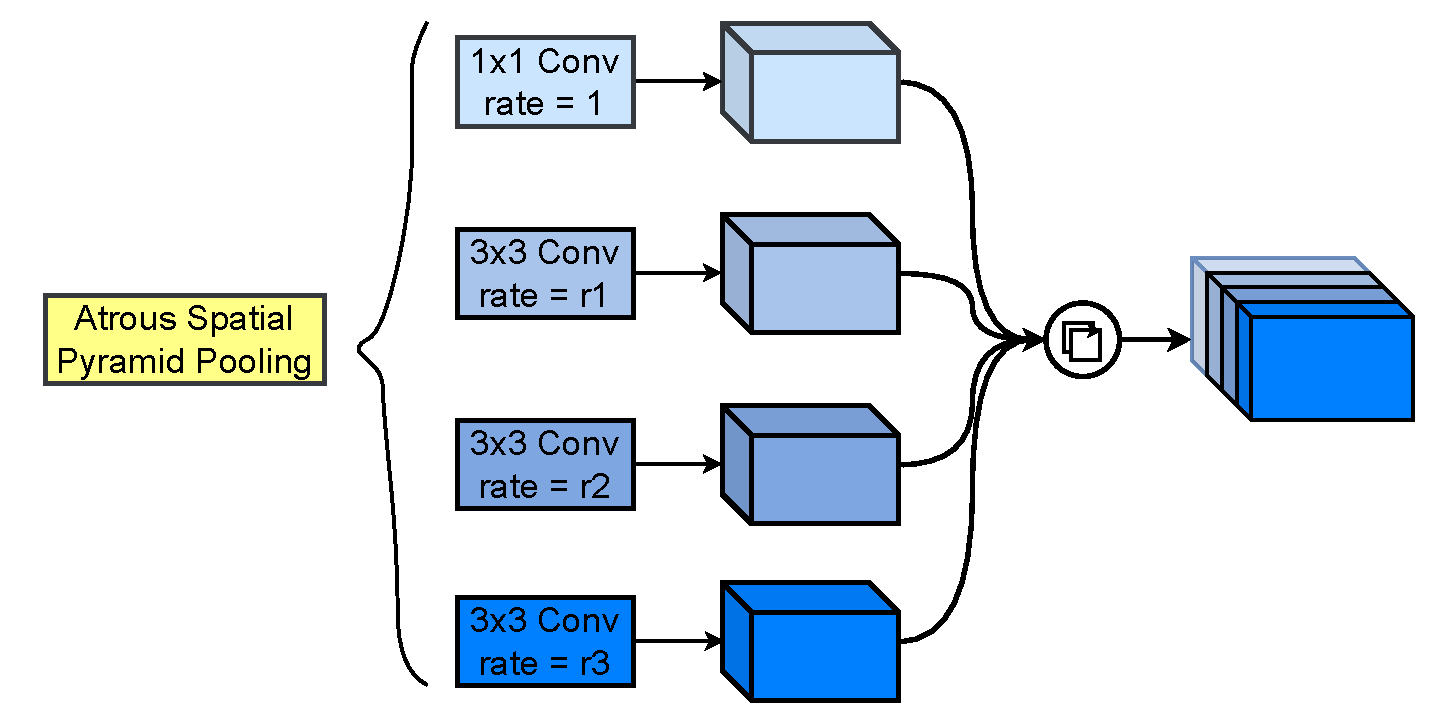
\includegraphics[width=0.4\textwidth]{img/Design-ASPP.pdf}
    \caption{Atrous spatial pyramid pooling module}
    \label{fig3}
\end{figure}

\begin{figure}[!t]
    \centering
    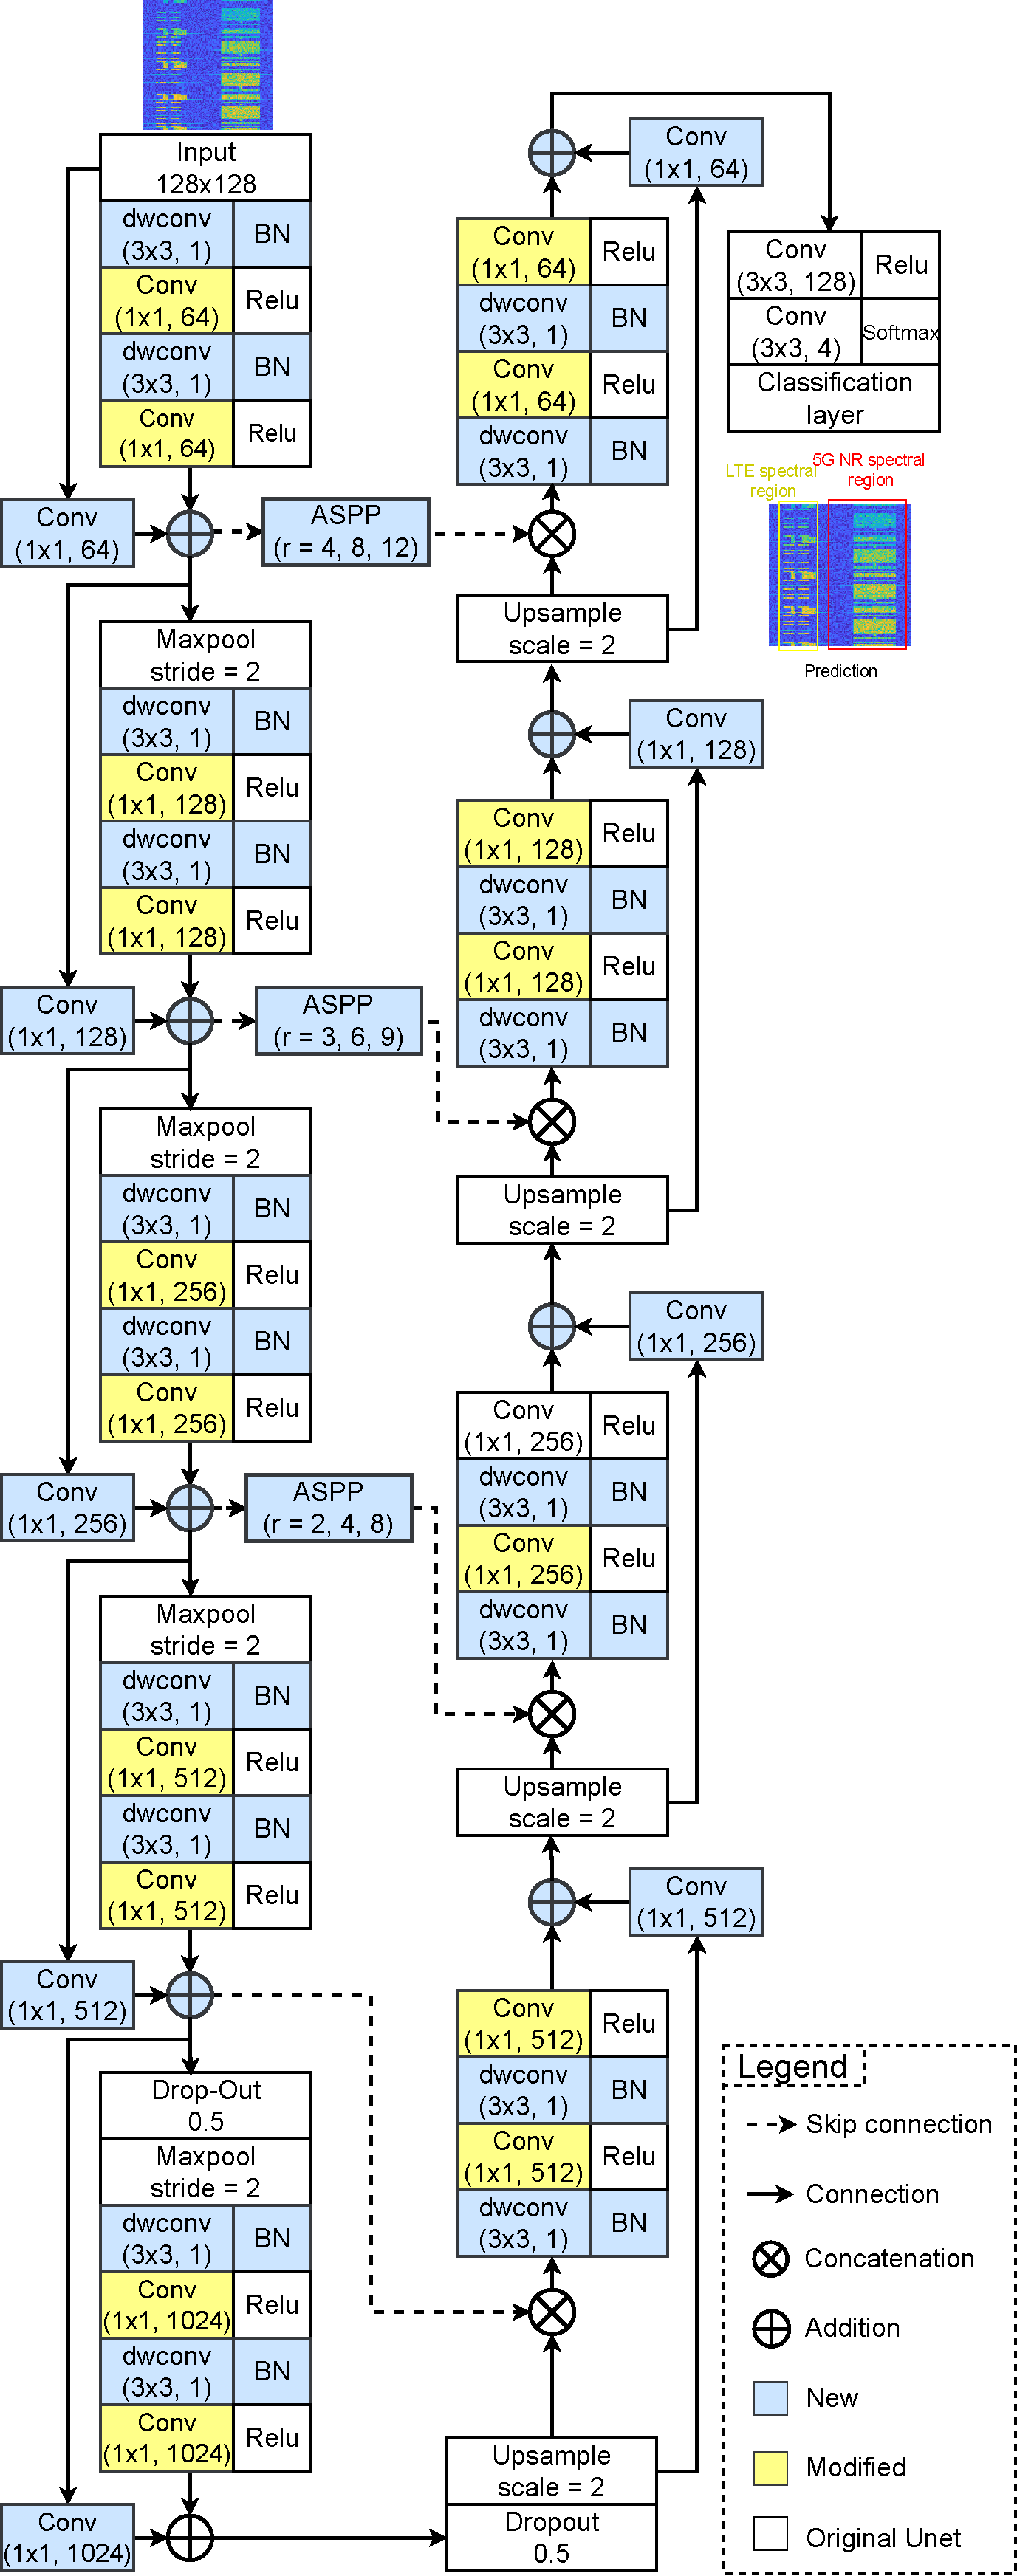
\includegraphics[width=0.4\textwidth]{img/Design-SpecSenseNet.pdf}
    \caption{Spectrum sensing network architecture}
    \label{fig4}
\end{figure}

The Fig. \ref{fig4} depicts SpecSenseNet architecture that is redesigned by Unet-based architecture \cite{ronneberger2015u}. SpecSenseNet comprises five layers for the encoder and decoder paths, ASPP is integrated into each skip connection path across multiple layers to enhance feature extraction across various scales. In detail, dilatation rates ($\mathrm{r_1, r_2, r_3}$) are $4, 8, 12$ in the first layer; $3, 6, 9$ in the second layer; and $2, 4, 8$ in the third layer respectively. Furthermore, we maintain a skip connection from the encoder to the decoder path in the last layer. Consequently, our proposed network offers the lowest complexity compared to original Unet architecture and other variants, it continues to uphold an impressive efficacy in image classification. By seamlessly integrating cutting-edge techniques, our model ensures a robust predictive capability, thereby underscoring its prowess in delivering accurate and efficient image classification outcomes. Following Table \ref{tab1} for network complexity comparison among our design with other architectures, SpecSenseNet decreases significant the number of parameters to $7.8$M, reducing by $75.1\%$ and approximately $81\%$ comparing to Unet and other variants (Unetp, UnetE, Unetpp), respectively. 


\section{Dataset, hardware resources, result and discussions}
\subsection{Dataset and training resources}
In this work, considering realistic challenges (e.g., cost and privacy), we use the 5G toolbox in MatLab to generate a synthetic 5G and LTE spectrum with three different types that include 5G, LTE, and overlapping 5G and LTE frames, respectively. In particular, the dataset contains $5,000$ samples in each type, $128 \times 128$ image size combines with SNR ranges in $[0, 30]$ dB. We divide the dataset to $80\%$, $10\%$, and $10\%$ for training, validation, and testing. In detail, training process is executed on a state-of-the-art computing system renowned for its high-performance capabilities, featuring a formidable $3.00$GHz central processing unit (CPU) combining with the cutting-edge graphic processing unit (GPU) RTX $2080$. Computing resources include a substantial $16$GB of memory capacity. Furthermore, training option establishes and initializes learning rate $0.001$, using $\mathtt{piecewise}$ for learning rate schedule. Training process is executed in $40$ epochs and validated every $1,000$ iterations. For more detailed information about the dataset and training resources, referring to Table \ref{tab2}.





\subsection{Simulation and evaluation result}
We evaluate networks in four metrics, which include global accuracy, average loss, weight intersection-over-union (IoU), and mean boundary F1 (BF) score. These metrics are widely used to evaluate the prediction ratio of semantic segmentation. Following to table \ref{tab3} for the detail information of our results. Weight IoU is a metric commonly used in the evaluation of semantic segmentation models by comparing the ground truth bounding box to the predicted bounding box. On the other hand, prediction is defined as the ability of a classification model to identify only the relevant data points, recall illustrates the ability of a model to find all the relevant cases within a dataset, and BF score is described as the harmonic mean of precision and recall for a classification model, respectively.

\begin{table}[!t]
\centering
\caption{Simulation result comparison}
\label{tab3}
\begin{tabular}{|c|c|c|c|c|c|}
\hline
\textbf{Network}  & \textbf{G.Accuracy (\%)} & \textbf{W.IoU (\%)} & \textbf{M.BFScore (\%)} \\
\hline
\textbf{SpecSenseNet}  & $97.233$  & $94.611$ & $87.320$  \\
Unet   & $98.227$   &  $96.539$ & $90.560$ \\
Unetp   & $98.070$   &  $96.245$ & $89.206$ \\
UnetE   & $97.844$   & $95.821$  & $88.056$ \\
Unetpp   & $97.981$   & $96.074$ & $88.892$ \\
ConvNet   & $39.696$  & $19.328$ & $15.612$ \\
Deeplabv3+   & $46.266$  &  $33.878$ & $14.397$ \\
\hline
\end{tabular}
\end{table}

\begin{figure}[!t]
    \centering
    \footnotesize
    \begin{tabular}{cccc}
        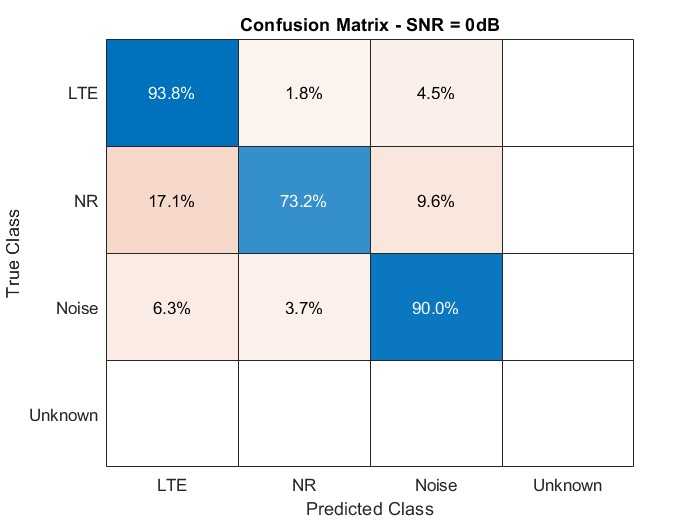
\includegraphics[width=0.24\textwidth]{img/confusion_matrix_0dB.jpg} & 
        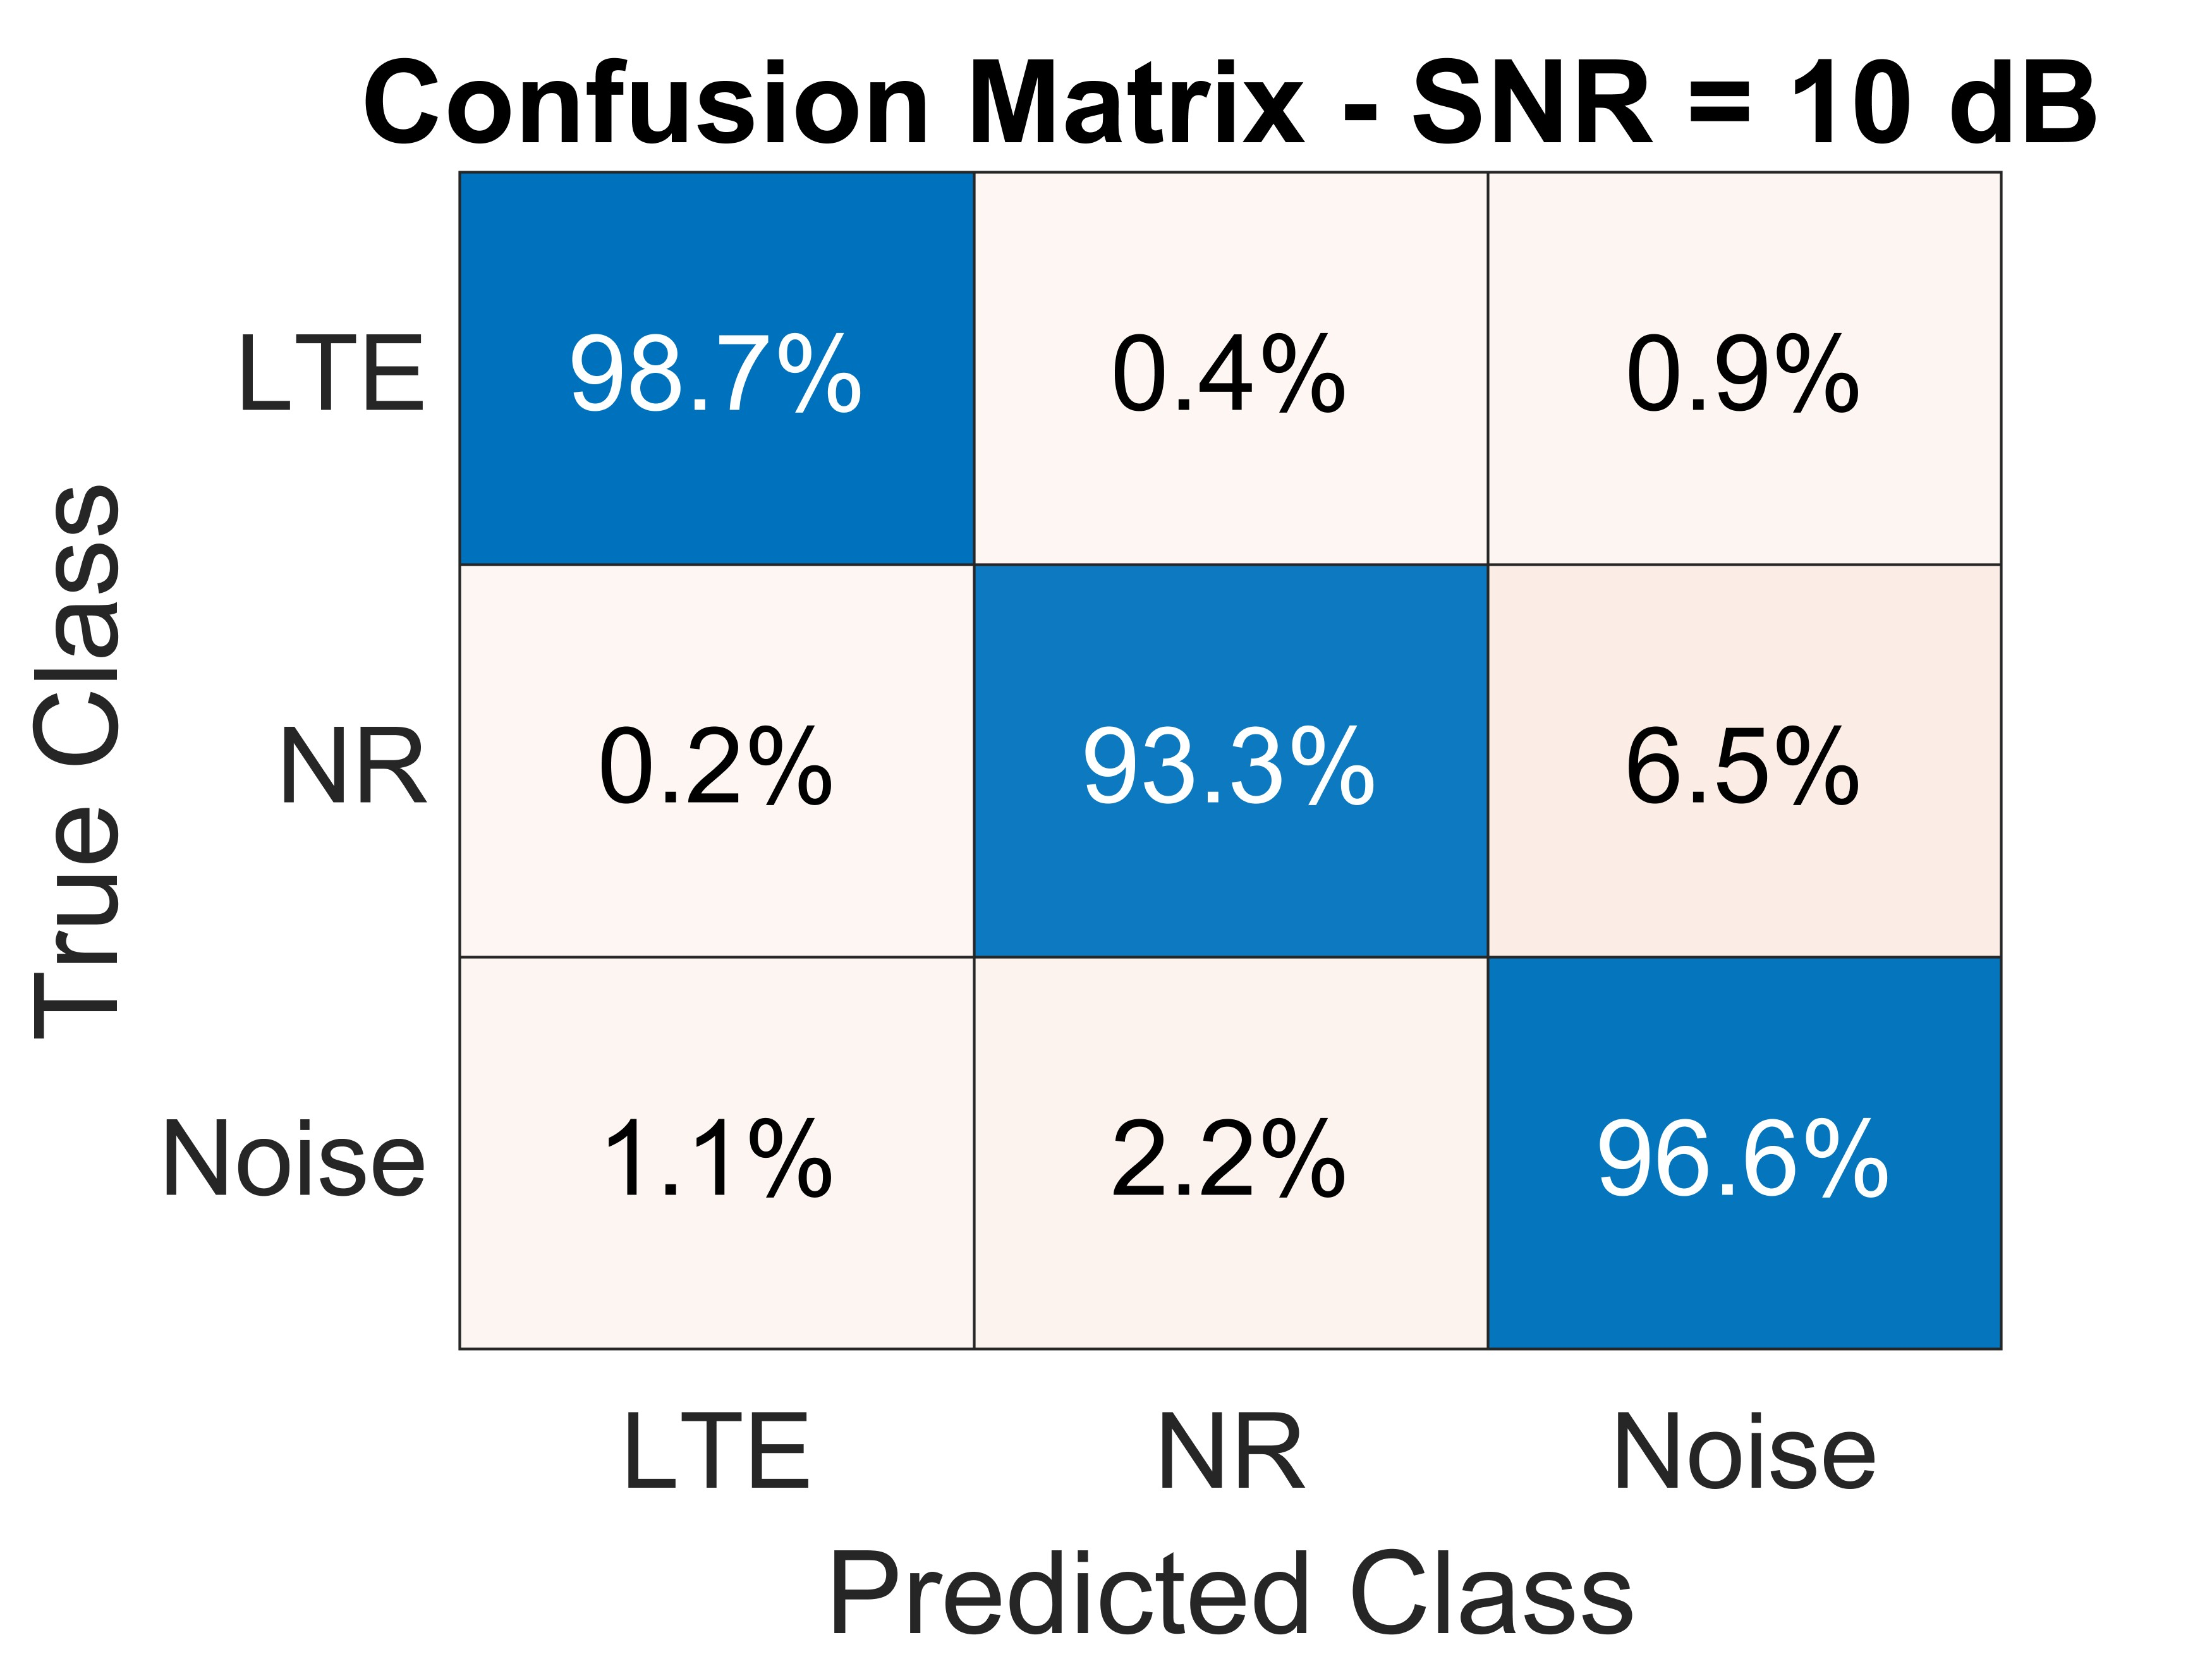
\includegraphics[width=0.24\textwidth]{img/confusion_matrix_10dB.jpg} & \\ (a) & (b) \\
        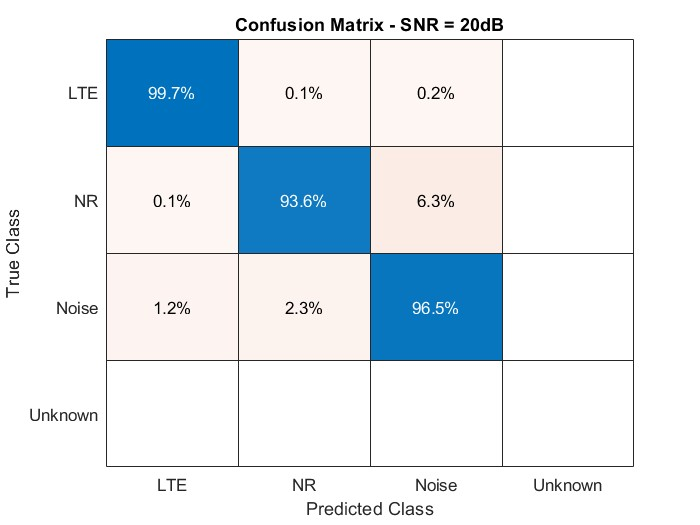
\includegraphics[width=0.24\textwidth]{img/confusion_matrix_20dB.jpg} & 
        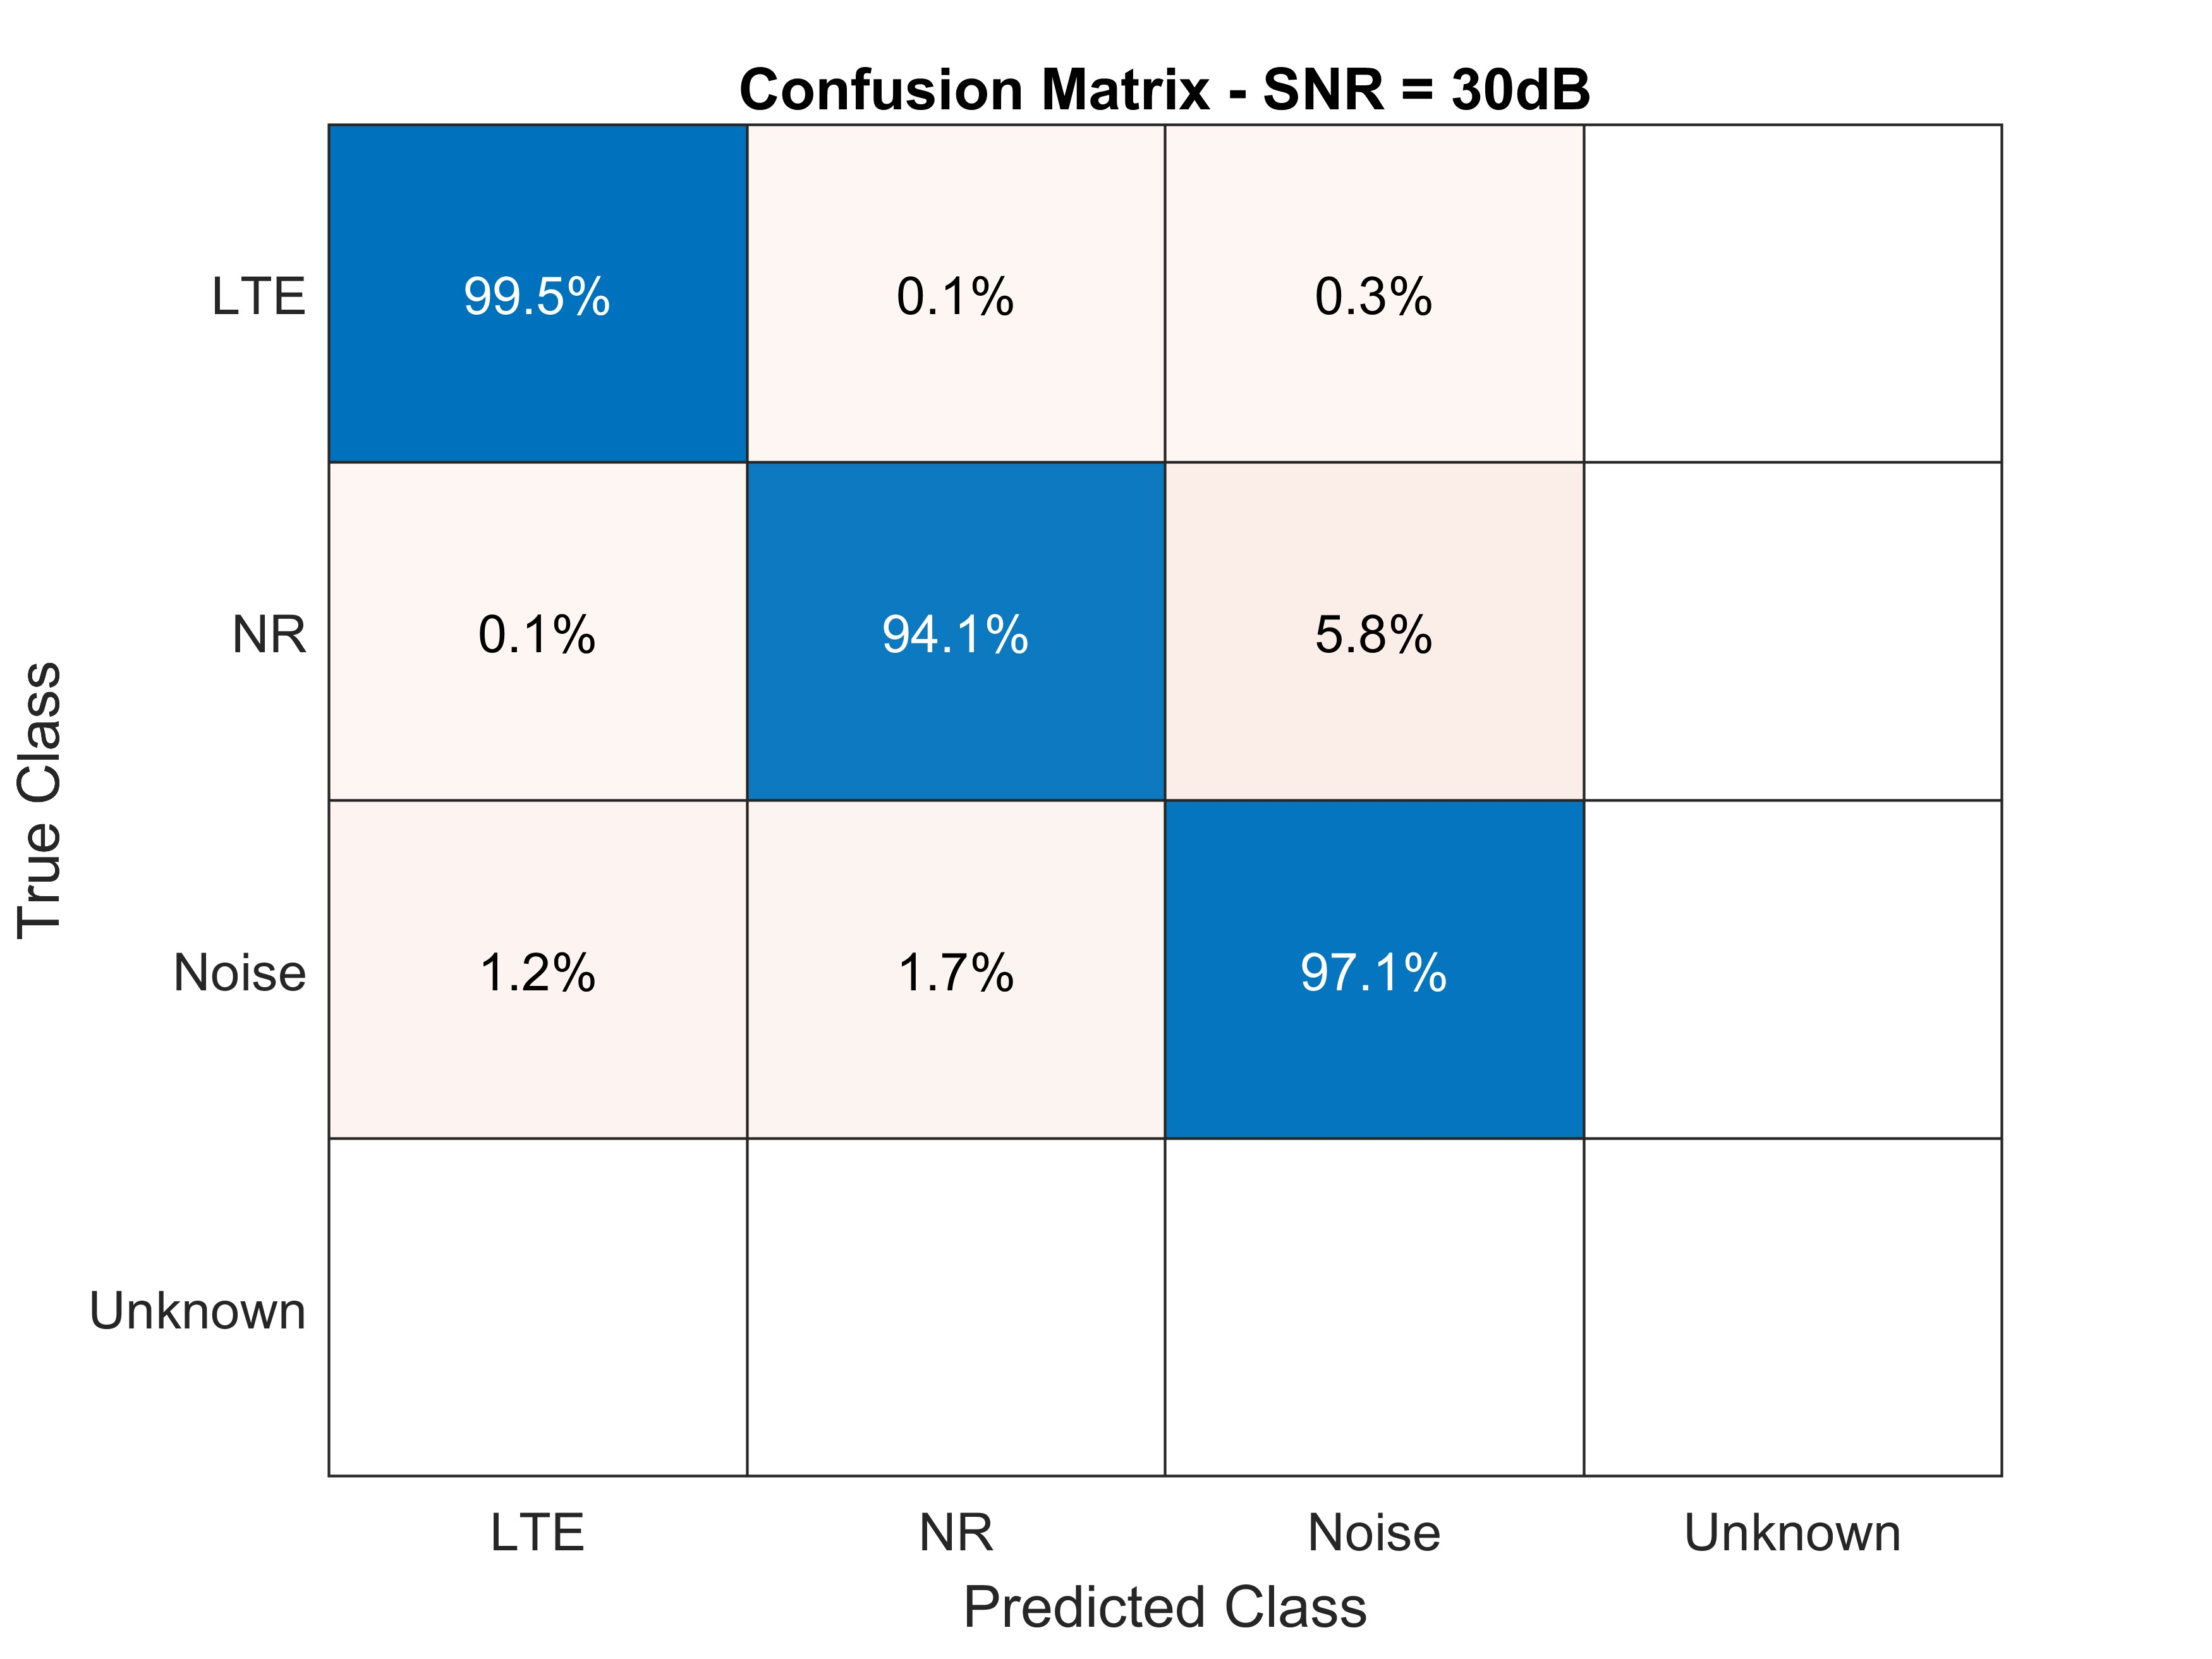
\includegraphics[width=0.24\textwidth]{img/confusion_matrix_30dB.jpg} & \\ (c) & (d)
    \end{tabular}
    \caption{Confusion matrix in different SNR levels: (a) $0$ dB, (b) $10$ dB, (c) $20$ dB, (d) $30$ dB}
    \label{fig5}
\end{figure}

\begin{figure}[!t]
    \centering
    \footnotesize
    \begin{tabular}{c}
        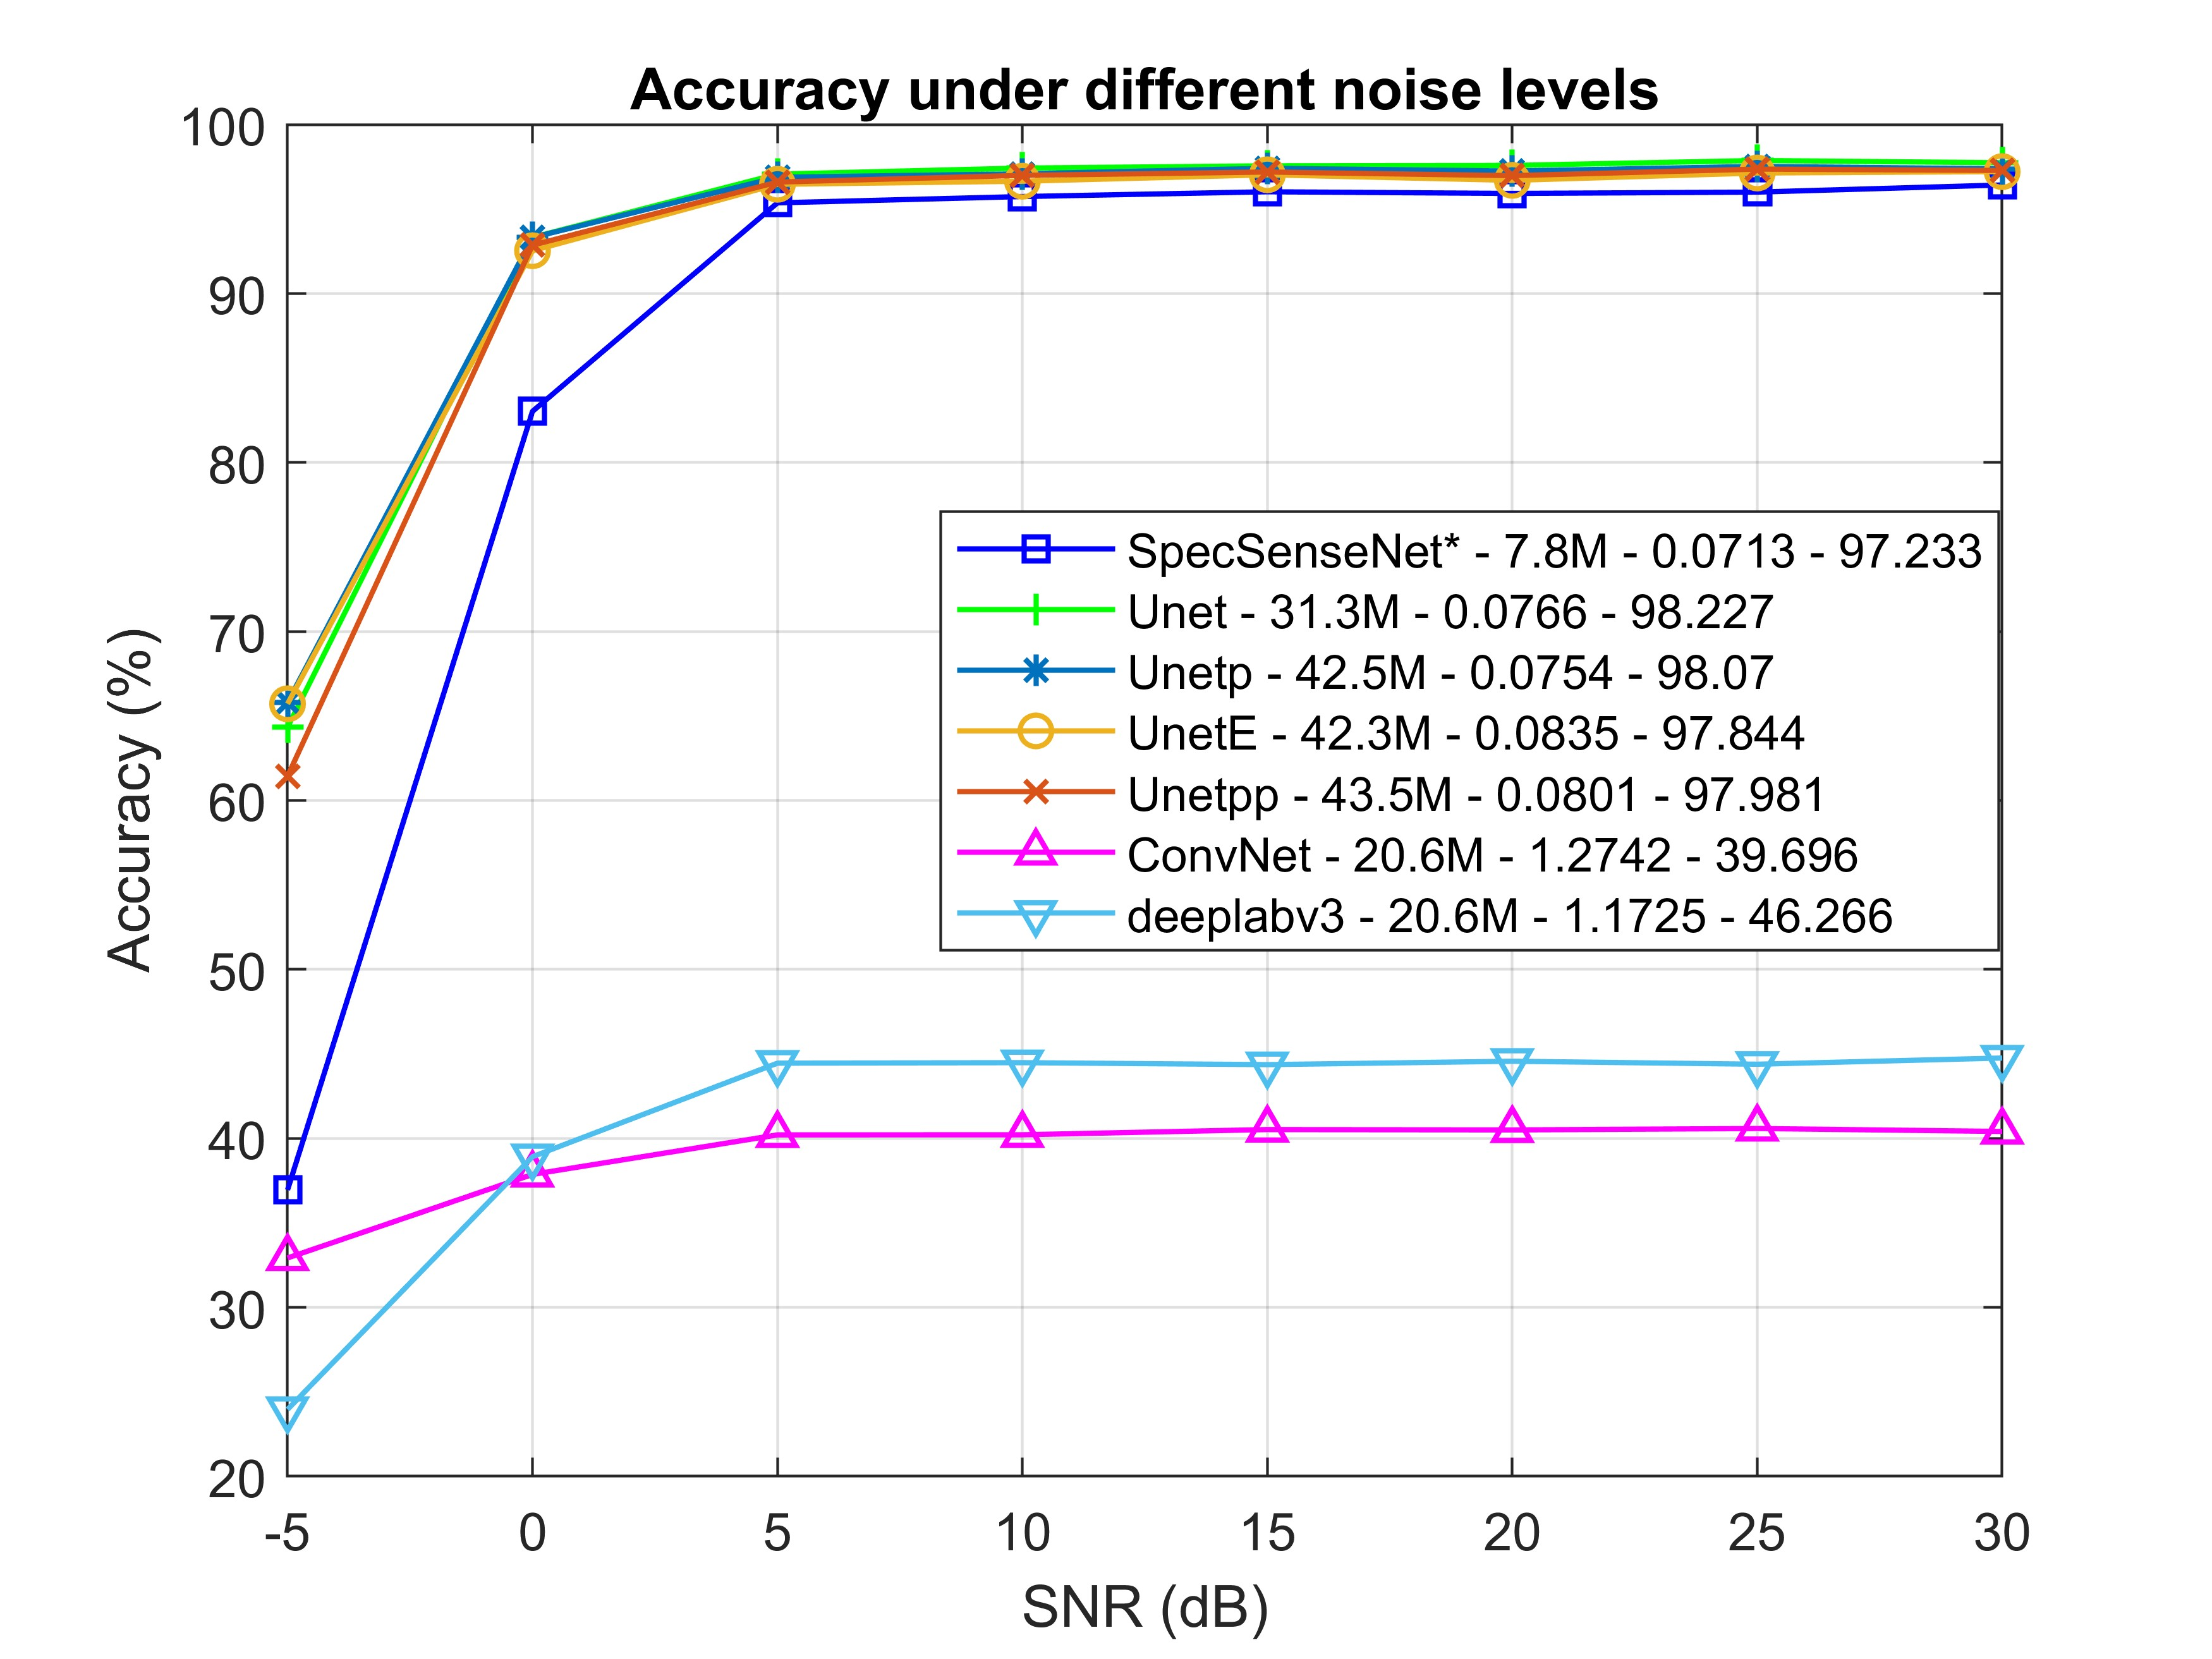
\includegraphics[width=0.4\textwidth]{img/accuracy_SNRs.jpg}
    \end{tabular}
    \caption{Accuracy evaluation under different noise levels}
    \label{fig6}
\end{figure}

\begin{figure}[!ht]
    \centering
    \footnotesize
    \begin{tabular}{ccc}
        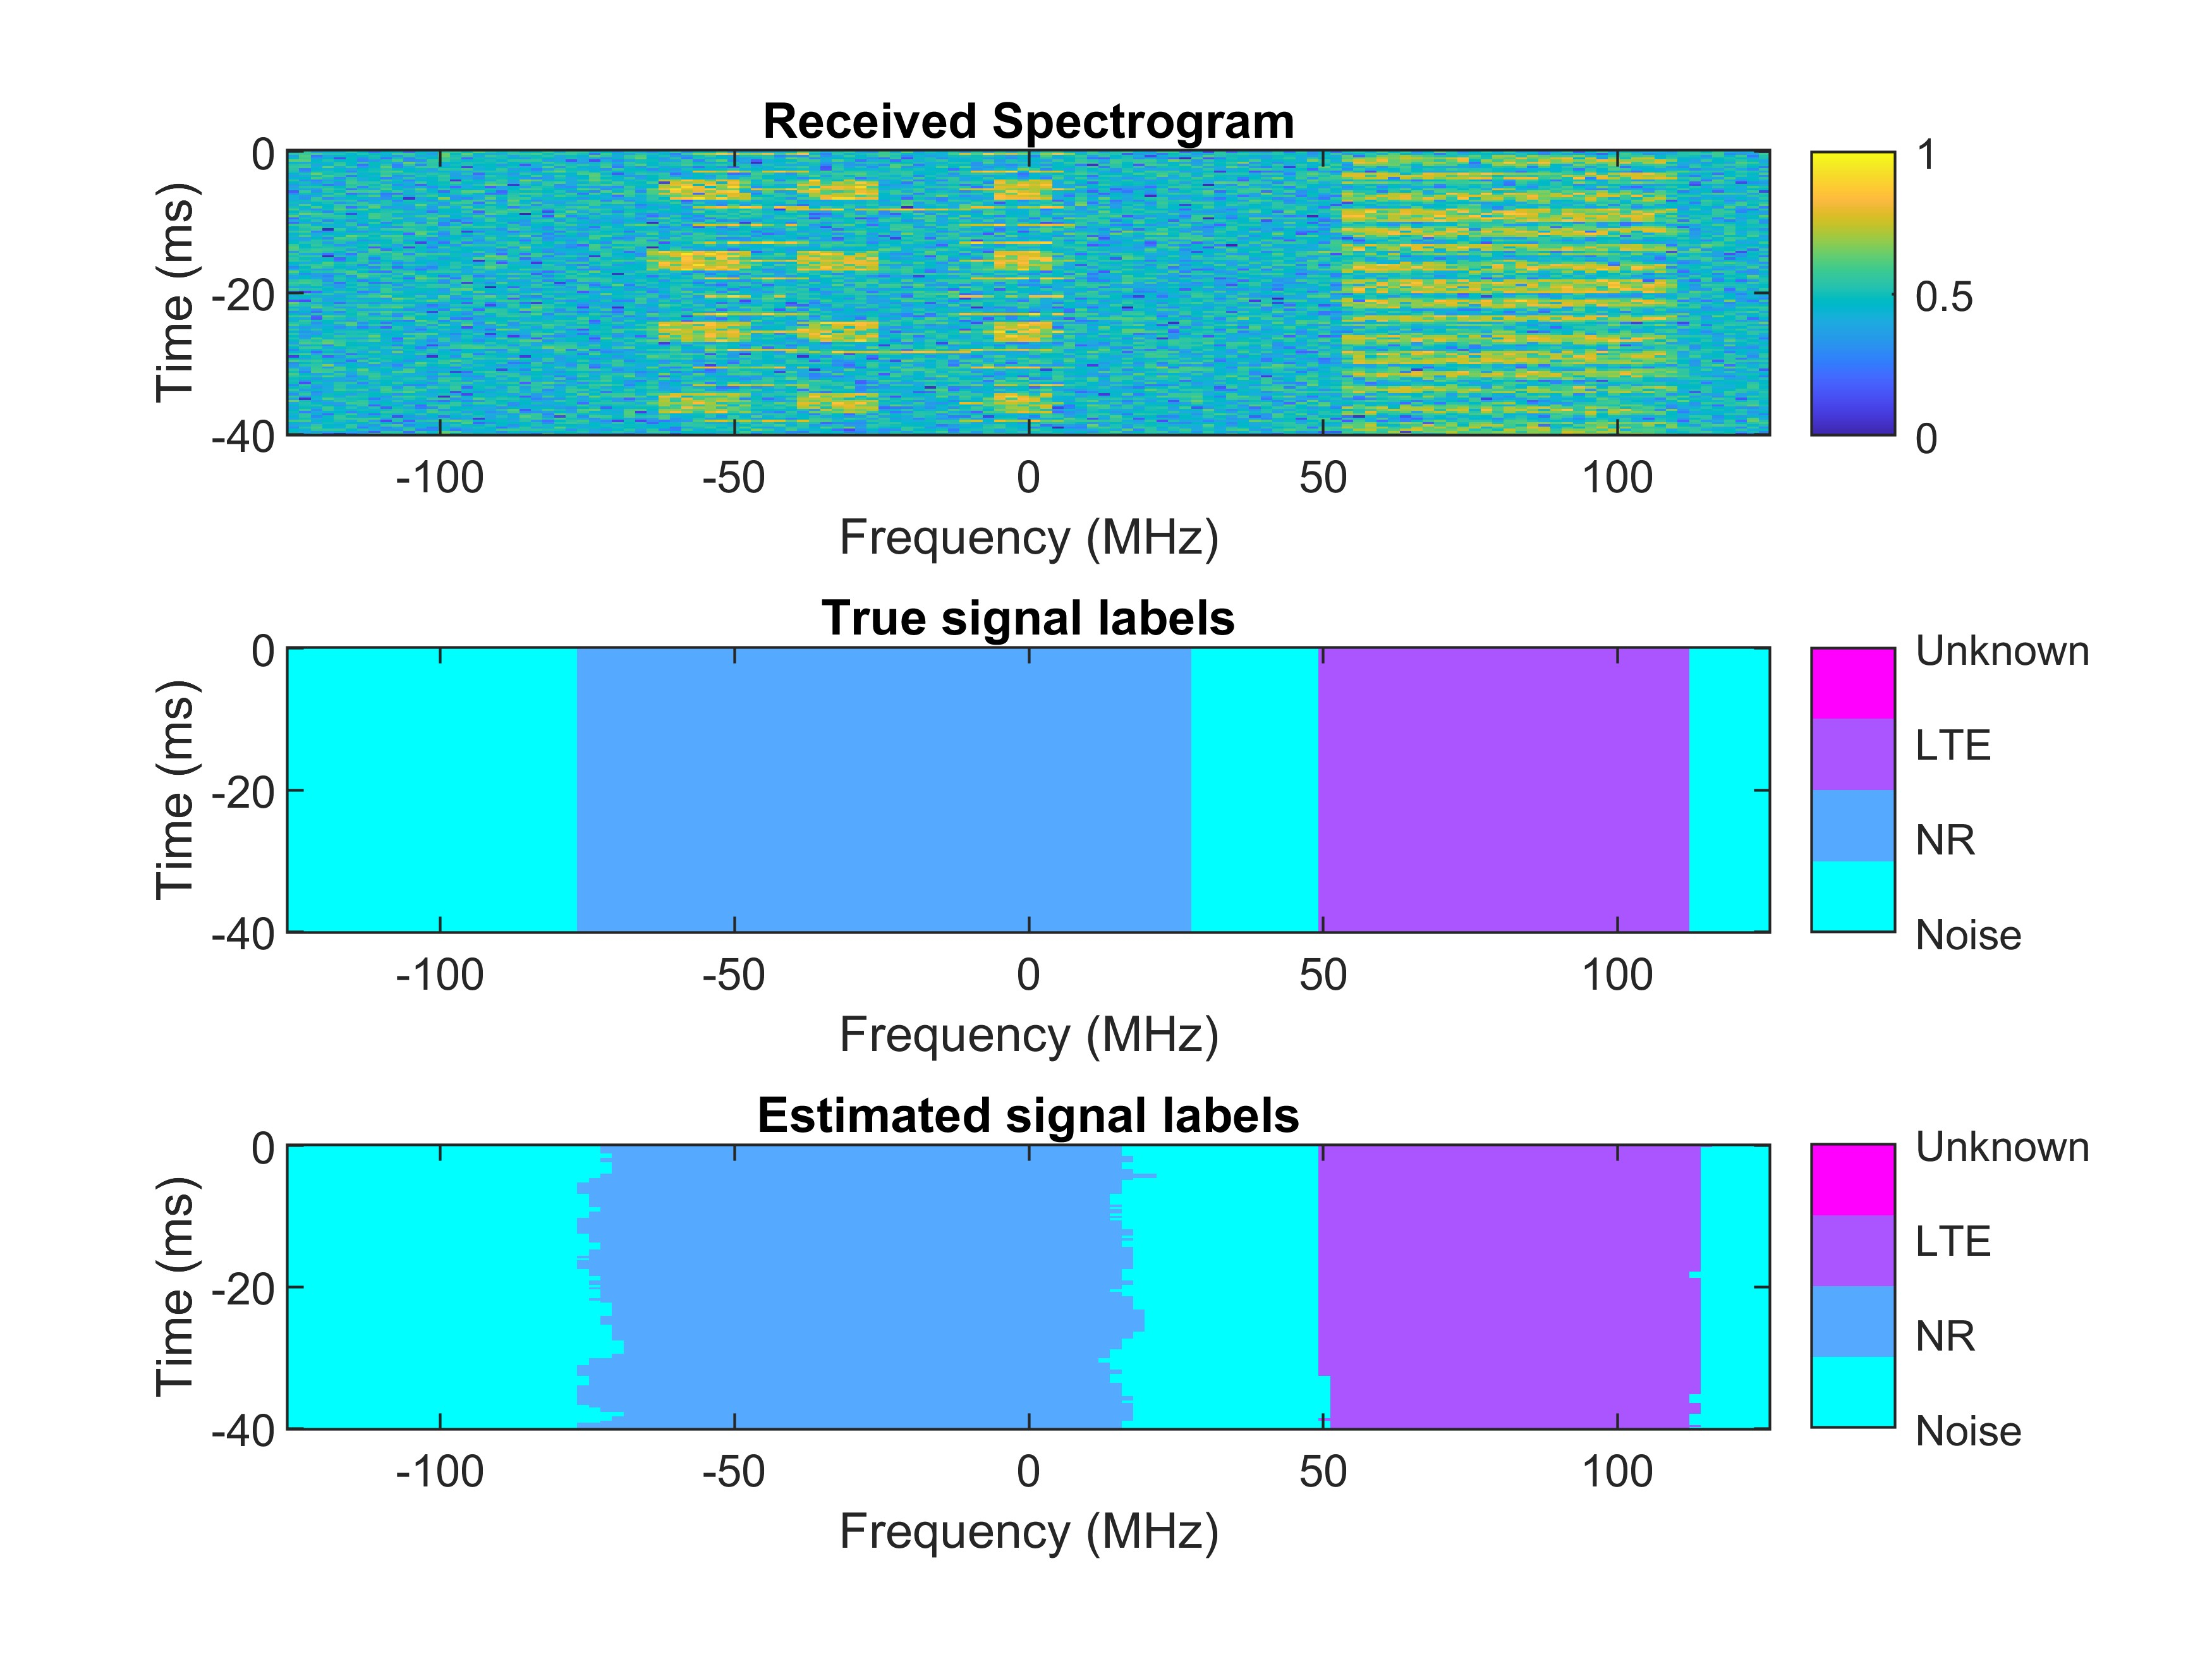
\includegraphics[width=0.45\textwidth]{img/Visualization_5dB.jpg} \\ (a)\\  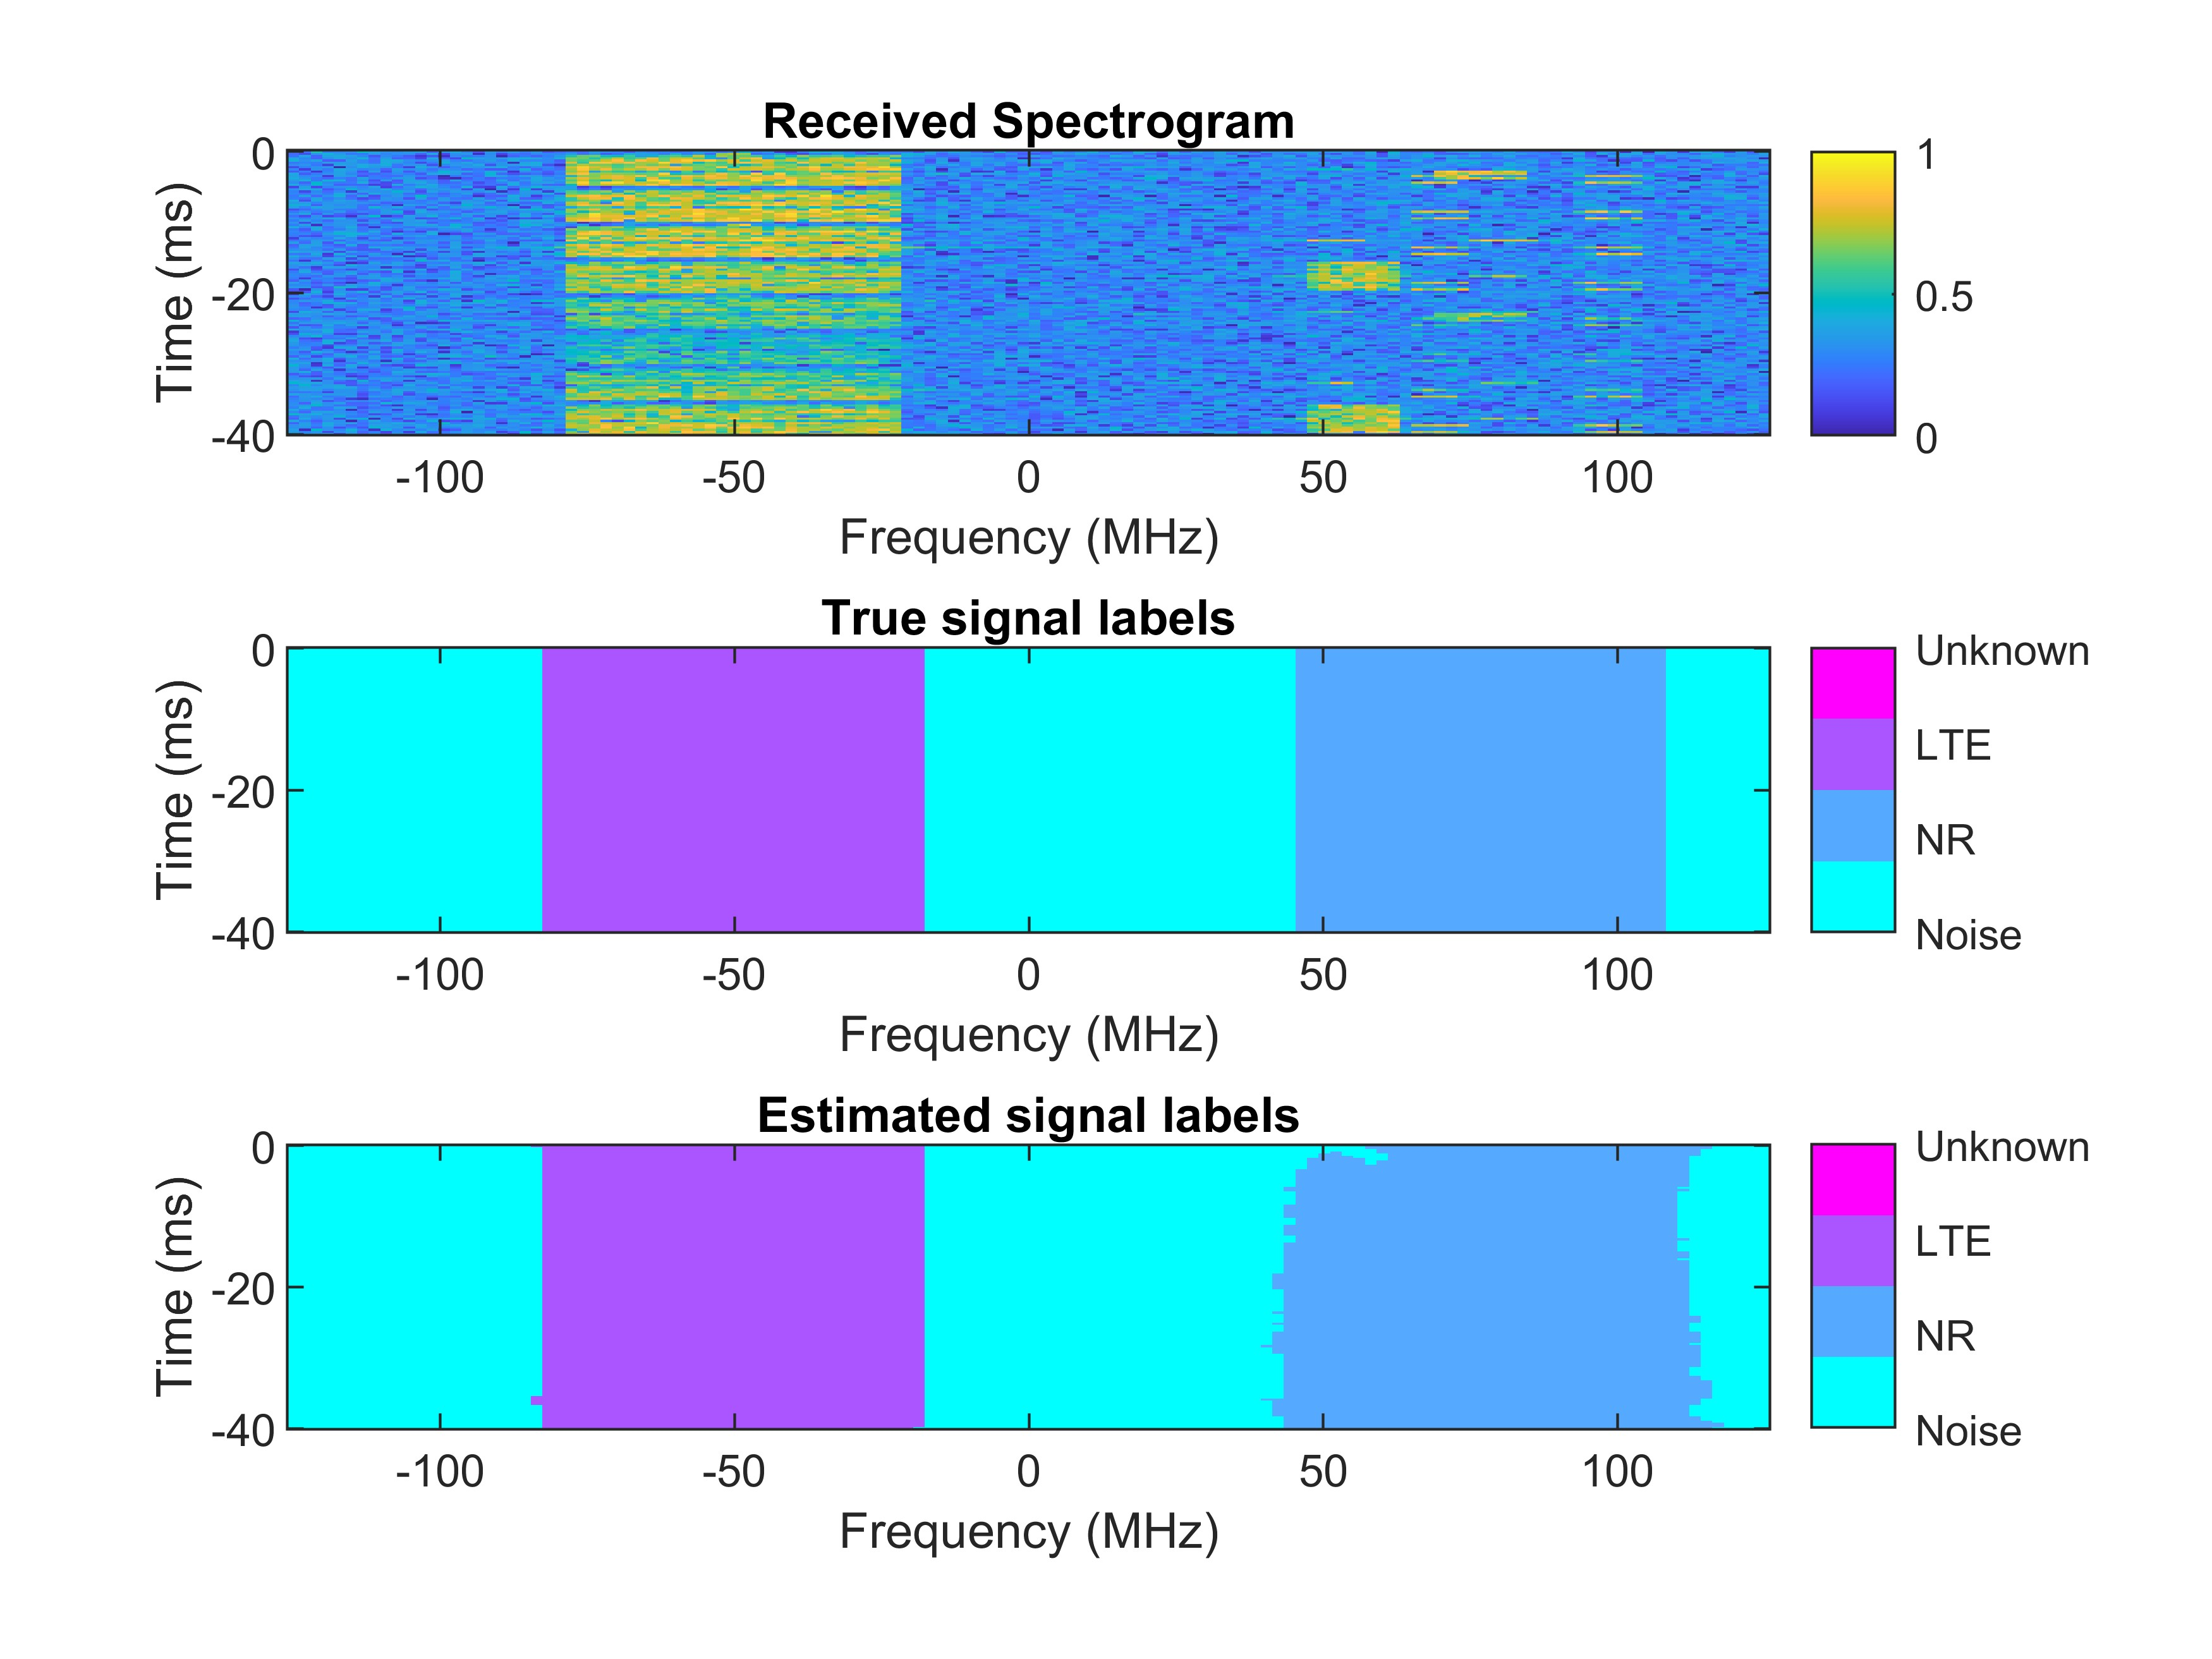
\includegraphics[width=0.45\textwidth]{img/Visualization_15dB.jpg} \\ (b)\\ 
        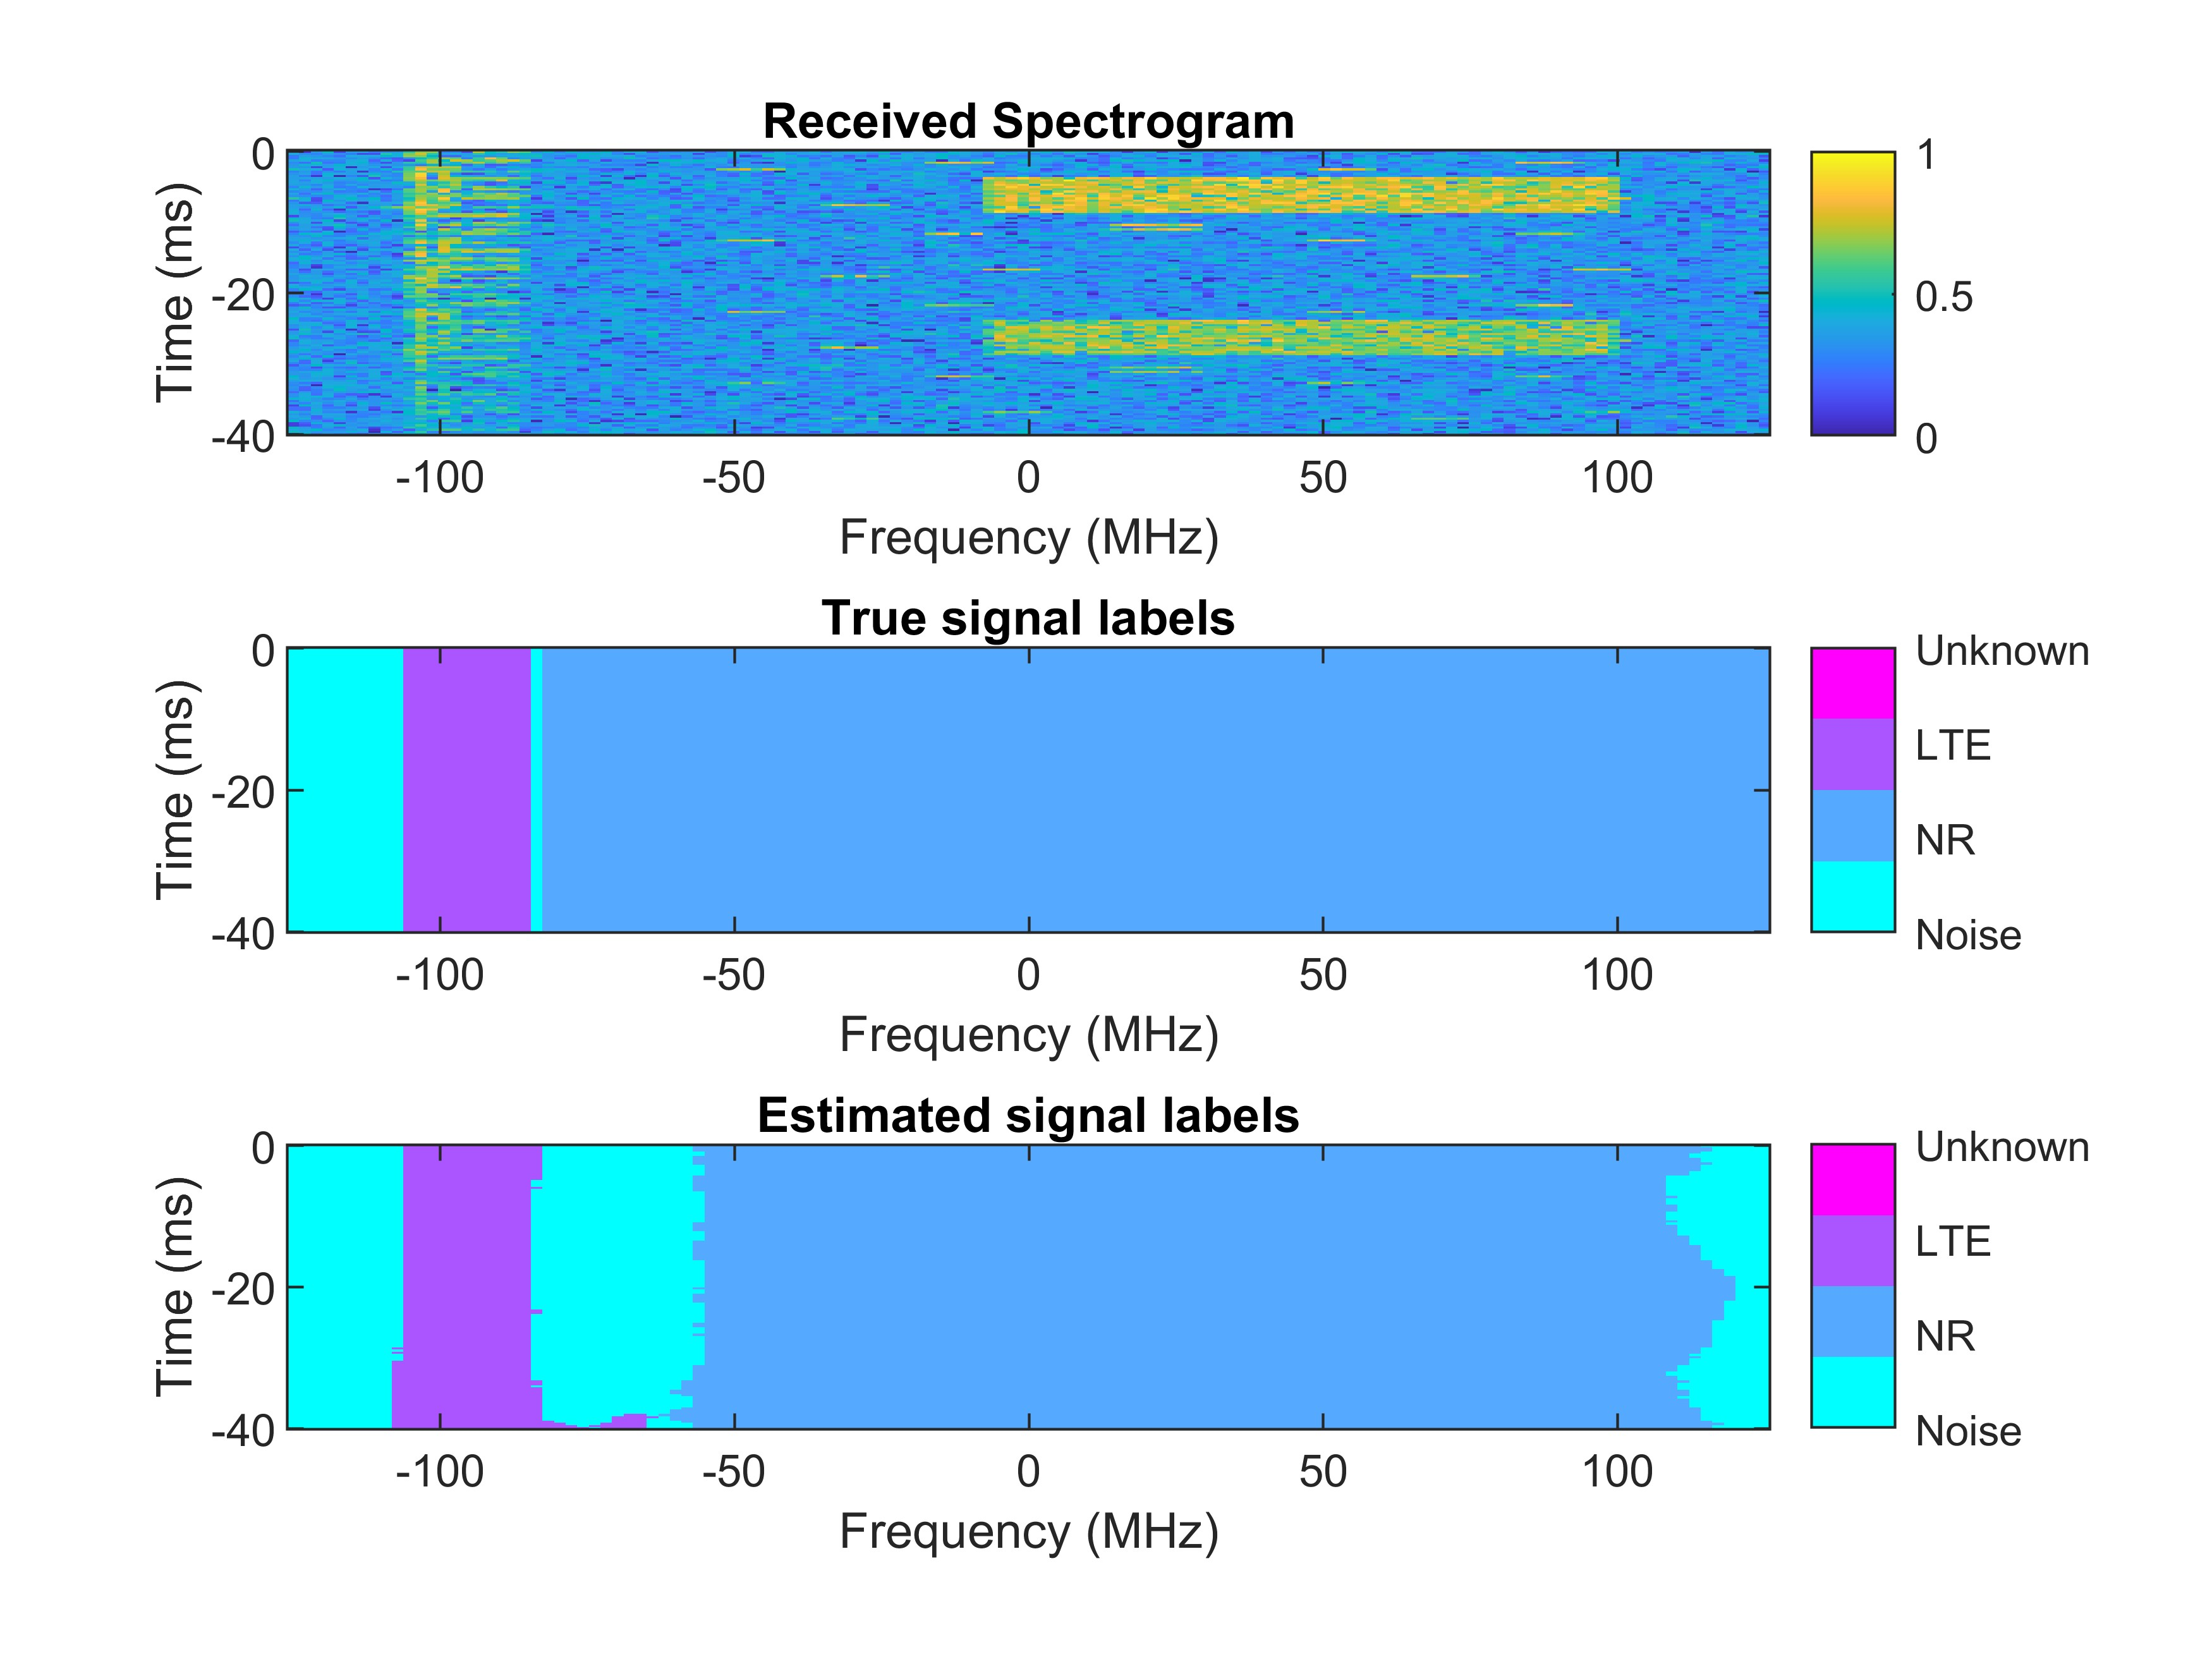
\includegraphics[width=0.45\textwidth]{img/Visualization_30dB.jpg} \\ (c)\\ 
    \end{tabular}
    \caption{Visualization of received spectrograms in various SNR levels: (a) $5$ dB, (b) $15$ dB, (c) $30$ dB}
    \label{fig7}
\end{figure}

In reference to Tables \ref{tab1} and \ref{tab3}, SpecSenseNet outperforms superior performance, achieving an impressive $97.223\%$ global accuracy. In comparison, ConvNet and Deeplabv3 exhibit considerably lower global accuracy of $39.696\%$ and $46.266\%$, respectively. Our proposal network consistently maintains a consistently high level of accuracy and performance, comparing to that of Unet-based architectures, while significantly reducing complexity. Specially, it achieves the same global accuracy while reducing the number of parameters by $75.1\%$, comparing to Unet. The Fig. \ref{fig5} and \ref{fig6} present confusion matrices generated during the evaluation of the SpecSenseNet model in different levels of additive noise, alongside the training accuracy evaluation process, comparing our model with others. Following confusion matrices, this study achieves notable outcome predictions across four distinct classes in various SNR levels. It is the fact that the performance of estimation labels increases corresponding to higher SNR levels, our network is estimated by test samples spanning various SNR levels, ranging $[-5, 30]$ dB. The consequence in Fig. \ref{fig6} depicts that our model acquires significant predictive accuracy across different SNR ranges, demonstrating a robust prediction performance, particularly at higher $5$ dB levels. In summary, these results demonstrate that SpecSenseNet substantially outperforms strongly semantic segmentation classification performance in all categories (i.e., 5G NR, LTE, noise, and unknown).

Regarding evaluation results in Fig. \ref{fig7} using several samples in various SNR levels, this work actually evaluates corresponding three overlapping 5G and LTE spectrogram samples at $5$ dB, $15$ dB, and $30$ dB respectively. Consequently, the classification accuracy improves comprehensively at all SNR ranges (e.g., the proportion of corrected prediction labels for 5G, LTE, noise and unknown signals). Respectively, with a $5$ dB of additive noise level, the prediction of labels is relatively accurate overall even though the gap estimation for 5G labels is only somewhat close compared to the true label. Nevertheless, it exhibits a significant improvement in classification results at $20$ dB, the gap label predictions are completely more accurate than that in $5$ dB. Particularly, achieving significantly accurate of predictions at $30$ dB, the performance gap between label estimations and ground true labels are completely close together. These consequences demonstrate that our network outperforms outstanding performance to apply for real-world applications.

\section{Conclusion}
In this paper, we presented an innovative SpecSenseNet utilizing Unet-based architecture, outperforming impressive performance in all different SNR levels of 5G and LTE spectrum sensing. Indeed, our study tackled performance problems when using DL for the spectrum sensing undertaking. Our proposed network reduced significantly complexity compared to Unet-based architectures and other variants, utilizing cutting-edge DL techniques to create a robust and cost efficient network. In summary, SpecSenseNet attained classification robustness base on simulation for spectrum sensing for 5G and LTE, combining with a high additive noise, making it suitable for real-world conditions. 

\bibliographystyle{IEEEtran}
\bibliography{reference}
\end{document}


